\documentclass[10pt,a4paper]{article}
\usepackage[utf8]{inputenc}
\usepackage{amsmath}
\usepackage{amsfonts}
\usepackage{amssymb}
\usepackage[hidelinks]{hyperref}
\usepackage{graphicx}
\usepackage{caption}
\usepackage{subcaption}
\usepackage{units} % For \nicefrac
\usepackage{algorithm2e} % For algorithms

\begin{document}

\title{SML World}
\date{2015}
\author{Rui Oliveira\\ Smart Mobility Lab, KTH}

\maketitle

\tableofcontents

\newpage

\section{Introduction}

The SML World is a tool for Autonomous Driving Research and Testing. It was created at KTH Royal Institute of Technology and it was developed to tailor the specific needs and capabilites of the Smart Mobility Lab.

This tool provides means of simulation, control, interaction and visualisation of autonomous vehicles in a realistic environment. This environment can be purely virtual, purely real, or a somewhere in between, since the system allows for the integration with scaled trucks located at the Smart Mobility Lab.

This document serves an introduction to the capabilities of the tool, and when deemed necessary it also explains important concepts in its implementation. It is the objective of the author that the reader gets a good understanding of the SML World after reading this document. The reader should also feel knowledgeable enough to start using (and improving) the SML World for one's own needs.

Section \ref{sec:the_sml_world} will give an introduction to the general structure of the SML World. The following sections will then go into the detail of the several modules that make the SML World run.

First we start by describing the Road Module in section \ref{sec:the_road_module}. This module is responsible for the road network processing.

The Simulation Module will be explained in section \ref{sec:the_simulation_module}. Here we specify how the car's dynamics and sensor readings are computed.

In section \ref{sec:the_v2v_module} we explain how vehicle-to-vehicle communication is achieved. We detail the two main modes of communication, globally, using network communications or locally using Wi-Fi communications.

The previous modules are enough to implement a simulation environment. By simply adding smart vehicles, as the ones explained in section \ref{sec:the_smart_vehicle}, we will finally have an autonomous driving simulator. However, one also wishes to see what is happening, cue the Visualisation Module, which is explained in section \ref{sec:the_visualisation_module}.

The next module to be described is specific to the Smart Mobility Lab, as it requires a Motion Capture System to work. Section \ref{sec:the_motion_capture_model}, explains the Motion Capture Module, and how it can be used to turn our computer simulation into a real life scaled simulation.

Finally in section \ref{sec:the_real_trucks_module} we explain the Scaled Trucks Module, which allows the usage of the scaled trucks present in the Smart Mobility Lab.


\graphicspath{ {SectionTheSMLWorld/Images/} }

\section{The SML World}
\label{sec:the_sml_world}

The whole system at play is referred to as the SML World. The SML World is mostly developed in Python, however it can have several auxiliary modules in different programming languages. In the past the SML World has distinct auxiliary modules written in languages such as Java, MATLAB, C++, LabVIEW and Unity, a game engine.

In this section we will explain the more general aspects of the SML World, and in future sections we will delve into the specific details and the auxiliary modules.

\subsection{The Vehicle Structure}
\label{subsec:the_vehicle_structure}

One of the fundamental pieces of a driving simulator would be, obviously, the vehicles, and our SML World will necessarily be populated with a multitude of those. We will describe the fundamental components of the vehicles that are implemented in the SML World.

\subsubsection{The Vehicle as an Object}

A vehicle in the SML World, will be implement as an instance of a Class, \textit{i.e.}, an object. In its most simple version, a vehicle will be an object composed only of attributes, and not implementing any method whatsoever.

\subsubsection{Vehicle Id}

Each vehicle will have an assigned id as an attribute. This id, will be a unique identifier, meaning that no more that one vehicle will have the same id. Non negative ids will be reserved for vehicles that are real, \textit{e.g.}, the scaled trucks in the SML. Virtual vehicles, \textit{i.e.} ,purely simulated vehicles, are then forced to have negative ids.

\subsubsection{Vehicle State}

Every vehicle can be described by its state. In its most simple form, a vehicle state can be composed of a position and a yaw angle, forming the state $(x,y,\theta)$. More complex vehicle models, can of course have higher dimensional states, and even include dynamics such as accelerations.

Every vehicle will store its state as a group of attributes, name according to the quantity/quality they are storing.

\subsubsection{Vehicle Commands}

Most vehicles can be controlled, \textit{i.e.}, a set of input commands can be applied to it, such that it can make an influence in its state. A simple example corresponds to a car vehicle, where the throttle and the steering directly influence the car state.

Vehicles having commands will store them as attributes named in accordance to their description.

\subsubsection{Vehicle Sensors}

A necessary requirement for autonomous driving is the usage of sensing technologies. Vehicles with equipped sensors will have an attribute corresponding to the readings performed by their sensors. This attribute is updated according to the current state of the vehicle and its surrounding environment.

\subsubsection{Vehicle Messages}

Cooperative autonomous vehicles might require communication to achieve cooperative driving. Vehicles requiring said functionality will have special attributes corresponding to communication buffers.

Each communicating vehicle will have two outgoing communication buffers, one for Network communications and the other for Wi-Fi communications. They will, of course, have the receiving counterpart, which will be composed of two incoming buffers corresponding to Network and Wi-Fi communications.

\subsubsection{Visualising the Vehicle Object}

Figure \ref{fig:vehicle_object} shows a visual representation of the vehicle object and its most fundamental attributes. To each vehicle running in the SML World a corresponding object will be used to represent it.

\begin{figure}[h!]
  \centering
    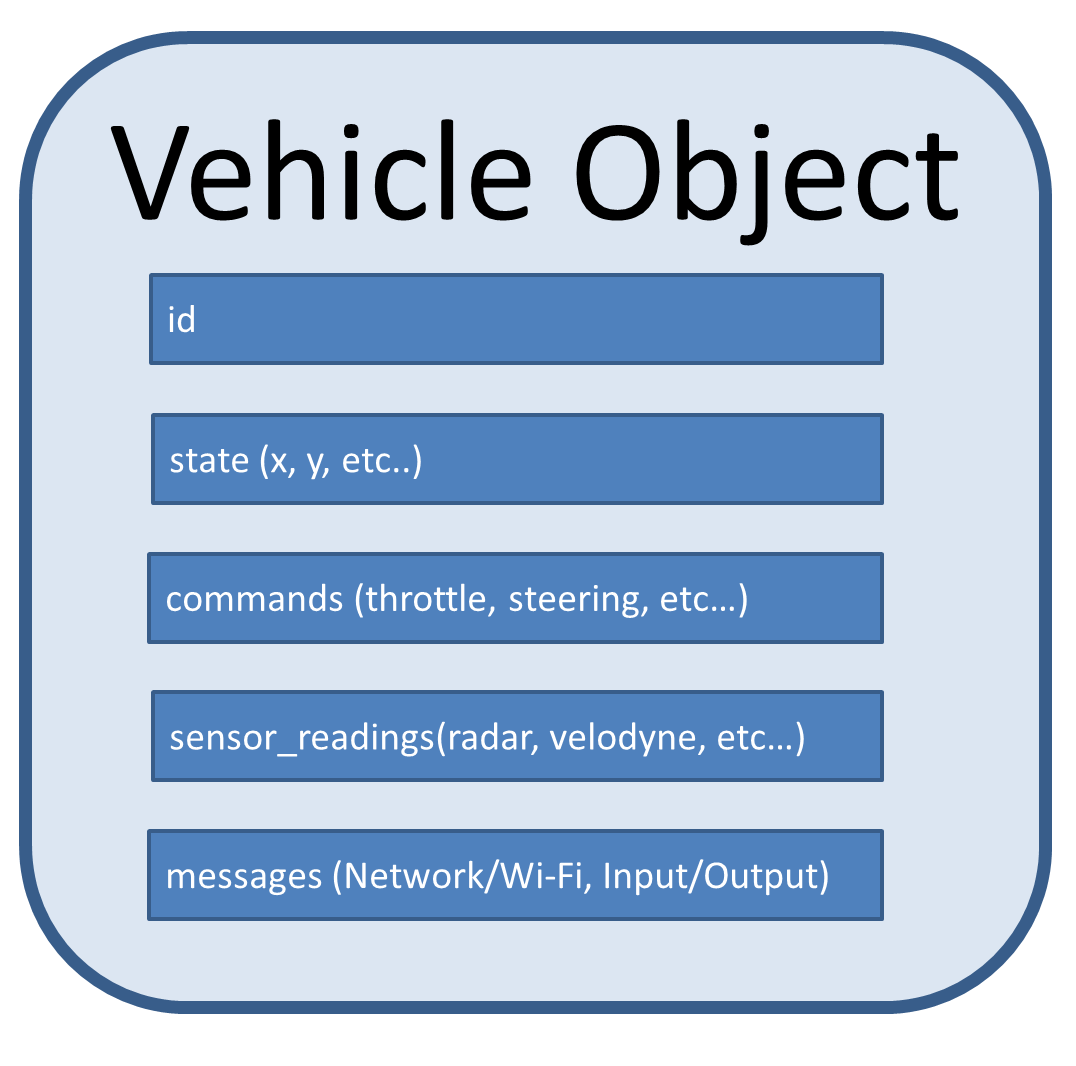
\includegraphics[width=0.6\textwidth]{vehicle_object}
    \caption{Representation of the vehicle object and its basic attributes \label{fig:vehicle_object} }
\end{figure}

\subsection{The SML World Structure}

An explanation of the SML World structure and its fundamental modules will be given here. The explanation will be as simplified as possible, however we will refer to the appropriate sections where these modules are explained in detail.

\subsubsection{The SML World Main Module}

The SML World in its simplest (and most useless form) simply consists of the main module running. This main module is simply used for storing information about vehicles in the world.

A simple depiction of it would be the one shown in figure \ref{fig:sml_world_structure_1}. In this figure, we use the block with name SML World to represent the main module of the SML World. In this module one can see a section of it called Vehicles Dictionary, this is the designation of the memory structure that contains all of the information about current vehicles in the SML World. Implementation wise it is achieved as a Python dictionary, hence the name. The keys of this dictionary are the ids of the vehicles in it. The values of this dictionary will be instances of the Vehicle Class, as explained in \ref{subsec:the_vehicle_structure}.

\begin{figure}[h!]
  \centering
    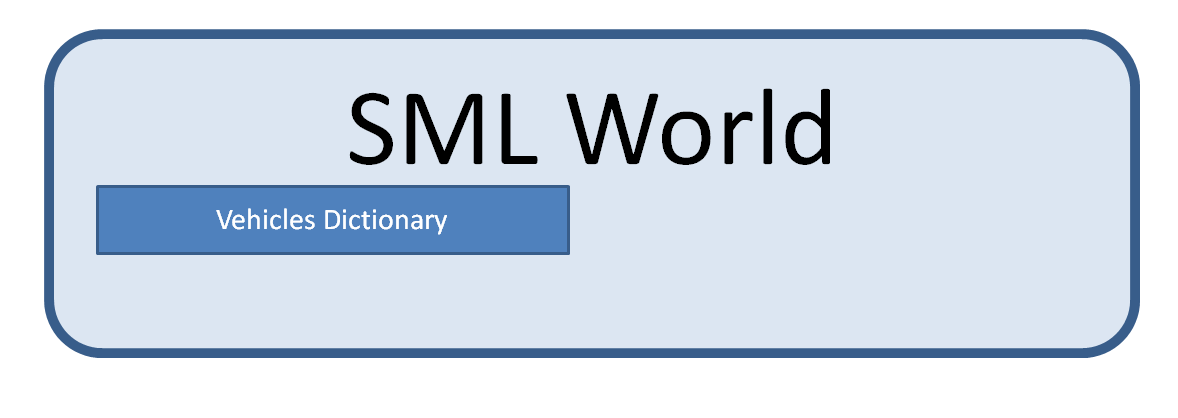
\includegraphics[width=1.0\textwidth]{sml_world_structure_1}
    \caption{The simplest form of the SML World, consisting only in the main module and the Vehicles Dictionary \label{fig:sml_world_structure_1} }
\end{figure}

\subsubsection{The Road Module}

We now add an extra component to our SML World, the Road Module. The Road Module is in charge of the road network, providing functionalities for visualisation and path generation for vehicles. A detailed explanation of it can be found in section \ref{sec:the_road_module}. With the addition of the Road Module the SML World now looks like the structure shown in figure \ref{fig:sml_world_structure_2}.

\begin{figure}[h!]
  \centering
    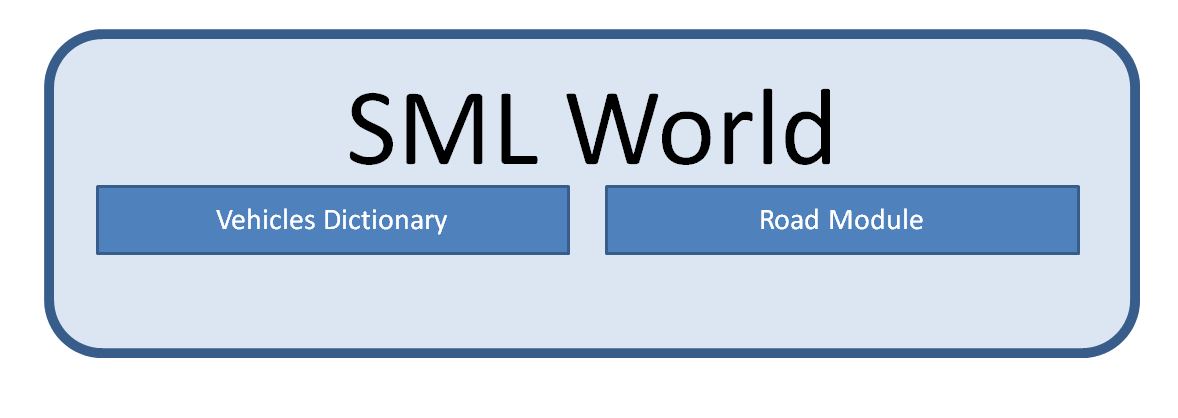
\includegraphics[width=1.0\textwidth]{sml_world_structure_2}
    \caption{The SML World, with the Road Module added \label{fig:sml_world_structure_2} }
\end{figure}

\subsubsection{The Simulation Module}

\label{subsubsec:simulation_module}

In its current state the SML World is able to store information about vehicles and the road network, as implemented by the Vehicles Dictionary and the Road Module. As is now, the SML World will simply be a static environment, as it is simply a container of information. We now add the Simulation Module so that we can get a dynamic world.

The Simulation Module, will be a Python class instantiated by the SML World, that will simulate the vehicles' movements. This class simply accesses the Vehicles Dictionary, and for each vehicle in it, it will perform a state (position, orientation, velocities, etc...) update based on the current state and the current vehicle inputs/commands (throttle, brake, steering, etc...). Besides the state update, the Simulation Module also updates the sensor readings (radar, velodyne, camera inputs, etc...) of each vehicle it simulates.

An important detail of the simulation module is that it is going to be running in parallel, that is, it will have it's own thread of execution. The simulation module will be running at a fixed rate, the higher this rate is, the more accurate the simulation is. A typical value for the simulation rate is somewhere around $50 Hz$.

Figure \ref{fig:sml_world_structure_3} shows the new structure diagram of the SML World with this added module. Notice that in the figure, the Simulation Module not completely contained within the SML World main module. We use this as a symbolic meaning that the Simulation Module is somewhat independent from the SML World, being that it is running on its own thread, but it still relies on it to perform it's task, since it needs to access and change the Vehicles Dictionary.

\begin{figure}[h!]
  \centering
    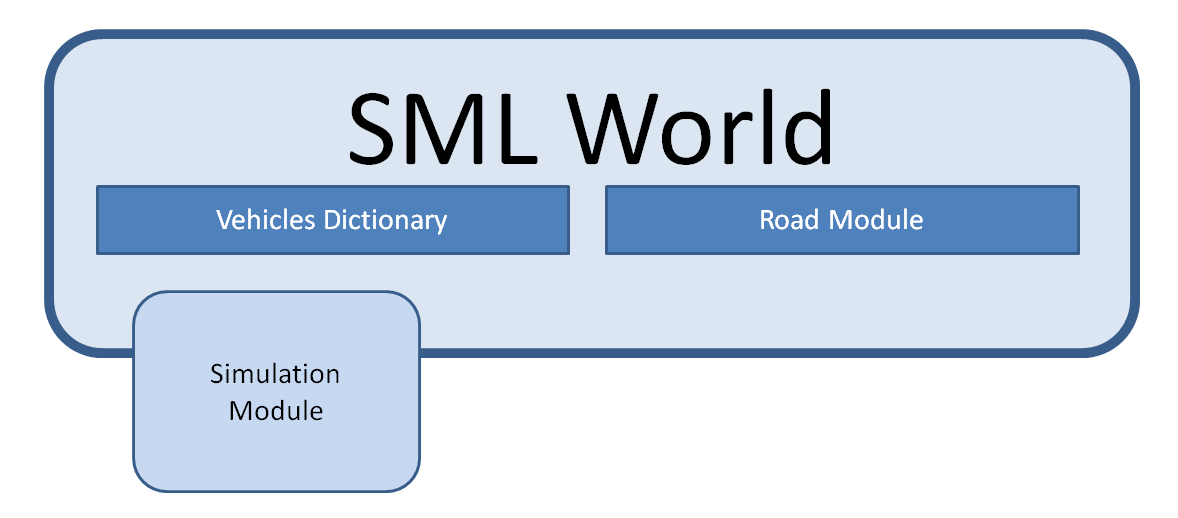
\includegraphics[width=1.0\textwidth]{sml_world_structure_3}
    \caption{The SML World, with a parallel execution thread corresponding to the Simulation Module \label{fig:sml_world_structure_3} }
\end{figure}


With this added module we now have a fully functional driving simulator, as vehicles can be simulated and their states updated according to the throttle and steering commands they have. If the vehicles in the Vehicles Dictionary already implement autonomous driving intelligence, then we can state that we already have a fully functional autonomous driving simulator.

\subsubsection{The V2V Module}

Currently we can achieve autonomous driving with the system as is, however if we wish to go one step further and allow for cooperative autonomous driving we need to provide the Vehicles with communications methods. To do so we use the V2V Module. V2V stands for Vehicle-to-Vehicle communication, and as the name implies it is used to allow vehicles to "talk" with each other.

The V2V Module implements this V2V communication, simulating two possible ways of communication, over the Network or over Wi-Fi. The V2V Module main task will be to make sure that outgoing messages of a vehicle are delivered to the respective vehicles they are destined to. To do so, this module will check the vehicles in the Vehicles Dictionary and update the incoming and outgoing messages that each vehicle has. A detailed explanation can be found in section \ref{sec:the_v2v_module}.

Similarly to the Simulation Module, the V2V Module will run in parallel, in it's own execution thread, at a fixed rate. The updated representation of the SML World structure can be seen in figure \ref{fig:sml_world_structure_4}.

\begin{figure}[h!]
  \centering
    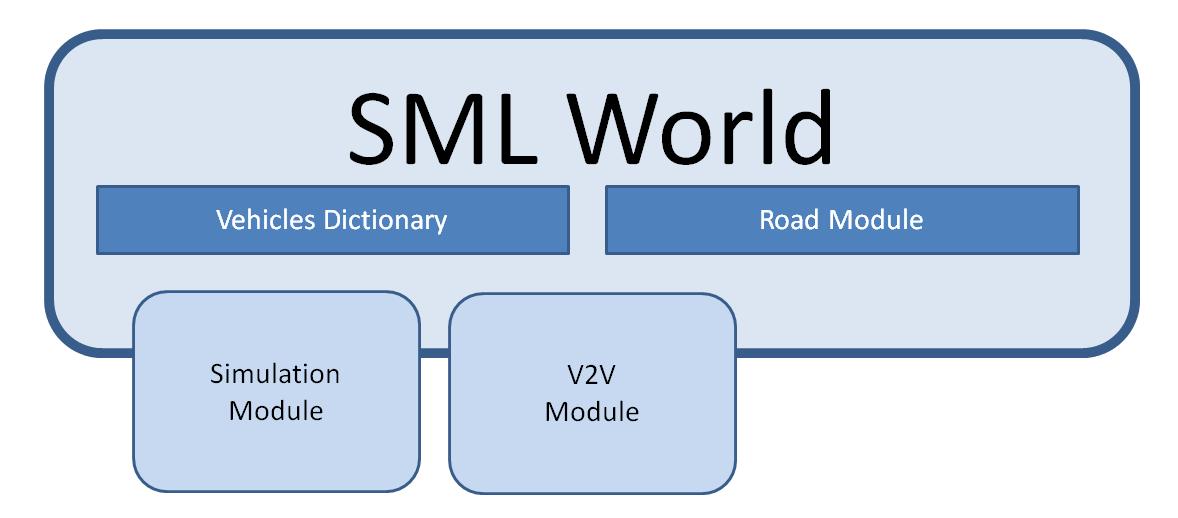
\includegraphics[width=1.0\textwidth]{sml_world_structure_4}
    \caption{The SML World, with a second parallel execution thread corresponding to the V2V Module \label{fig:sml_world_structure_4} }
\end{figure}


\graphicspath{ {SectionTheRoadModule/Images/} }


\section{The Road Module}
\label{sec:the_road_module}



\subsection{Introduction}

The first step when using the SML World, is to set up the environment to be simulated. This environment consists in the definition of the roads where the cars can move, and how the environment looks (forest areas, dirt areas, river areas, etc...).

In this document two different things will be explained, in section \ref{sec:theroadnetwork} the construction and definition of the environment is explained. Section \ref{sec:roadmodule} explains how this environment can be used/interfaced with in the SML World.


\subsection{The Road Network}
\label{sec:theroadnetwork}

The road network determines the road setup and how can cars move in it. The road network definition is based on the ideas implemented in OpenStreetMap \cite{OSM}. The goal of the OpenStreetMap project is to provide a free geographic data, and allow users to contribute for the improvement of said maps.

\subsubsection{A quick introduction to OpenStreetMap}

The information here given is mostly taken from the OpenStreetMap Wiki page, more detailed information can be found there.

OpenStreetMap is based on three fundamental elements, nodes, ways and relations.

\begin{description}
  \item[Nodes] A node is an individual point on a map. Associated to each point is a set of GPS coordinates, latitude and longitude, and a unique indentifier, an id. Two or more nodes can be connected together to form complex shapes. This is done making use of ways. Figure \ref{fig:osm_nodes} shows a group of nodes.
  \item[Ways] A way is a line of nodes. This line is formed by connecting the nodes belonging to the way through straight segments. Several different ways can be formed with the same set of nodes, the order of the nodes in the way is then essential for it's correct definition. Ways can close on themselves, forming closed ways. Closed ways can be useful to define areas or regions. Figure \ref{fig:osm_way} shows an example of a way, notice that the way has a defined direction, if the nodes were ordered in reverse, the direction would be the opposite.
  \item[Relations]A relation is used to described more complex concepts that might involve multiple ways. That said a relation can be thought of as a grouping of ways, just like a way is a grouping of nodes. A relation is composed by it's members, and their roles in the relation.
\end{description}

\begin{figure}[h!]
  \centering
    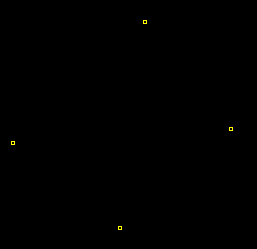
\includegraphics[width=0.5\textwidth]{osm_nodes}
    \caption{Visualisation of four nodes (visualisation using JOSM) \label{fig:osm_nodes} }
\end{figure}

\begin{figure}[h!]
    \centering
    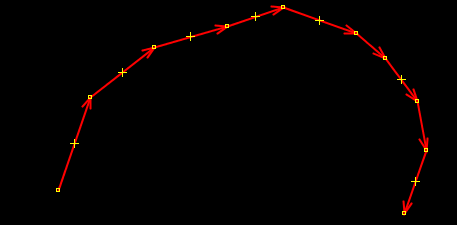
\includegraphics[width=0.5\textwidth]{osm_way}
    \caption{Visualisation of a way made up of ten nodes (visualisation using JOSM) \label{fig:osm_way} }
\end{figure}

Furthermore each of these elements can have tags. A tag is simply extra information that can be added to every element. A tag is defined by its name and value.

Making use of the simple concepts explained previously it is possible to define very complex maps.

\subsubsection{Adapting OpenStreetMap to the SML World}

In order to define our SML World road network, we will make use of the OpenStreetMap elements, however some additional concepts/conventions have to be defined.

\paragraph{Introduction to Lanelets}

Lanelets are the main concept used when defining the SML World road network. A lanelet is a particular case of an OSM Relation and it defines a road lane. Any road lane is defined by its limits (left and right lane markings). Road lanes also need a direction to be defined (unless they are bi-directional).

The creation of a lanelet is as follows:

\begin{enumerate}
\item Create the way (and respective nodes) corresponding to the left lane markings
\item Create the way (and respective nodes) corresponding to the right lane markings
\item Create a relation, and add as members the previous ways, with the respective roles, left\_lane\_marking and right\_lane\_marking
\end{enumerate}

The direction of the lanelet is defined by the direction of the right\_lane\_marking way. Whatever the direction of left\_lane\_marking might be, the direction of the lanelet will be the same as the direction of the right\_lane\_marking way.

Let us imagine we wish to define the road shown in figure \ref{fig:road_to_define}. These road is section is composed of two lanes, and as such we will need two lanelets to define this road. First we need to define the ways, that correspond to the left and right lane markings. In order to create these ways, we need first to add the corresponding nodes. Figure \ref{fig:road_to_define_with_nodes} shows the nodes that need to be created in order to define the ways corresponding to the lane markings. Once these nodes are added, we simple create the respective ways, as shown in figure \ref{fig:road_to_define_with_ways}. The orange and pink ways, will be the right\_lane\_marking of each lanelet, whilst the blue way will be the left\_lane\_marking of both lanelets. Note that the direction of the right lane marking will always define the direction of the lanelet, and as such it is important that this way is correctly oriented. It might be confusing that the same way, and the same direction, is used for the left\_lane\_marking of both lanelets, but this will not be a problem, as we simply use the left\_lane\_marking of a lanelet to know where a lane boundary is, not its direction.

\begin{figure}[h!]
  \centering
    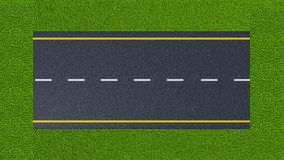
\includegraphics[width=0.5\textwidth]{road_original}
    \caption{The road section that we wish to define \label{fig:road_to_define} }
\end{figure}

\begin{figure}[h!]
    \centering
    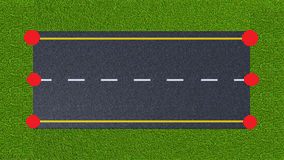
\includegraphics[width=0.5\textwidth]{road_with_nodes}
    \caption{Road section overlayed with necessary nodes \label{fig:road_to_define_with_nodes} }
\end{figure}

\begin{figure}[h!]
    \centering
    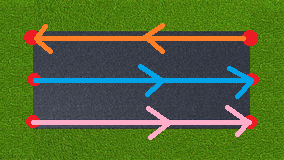
\includegraphics[width=0.5\textwidth]{road_with_ways}
    \caption{Road section overlayed with necessary ways \label{fig:road_to_define_with_ways} }
\end{figure}

\paragraph{Defining a Road Network using Lanelets}

A road network can be created making use of several lanelets. First however we need to define the concept of Lanelet Adjacency.

\textbf{Lanelet Adjacency} Two lanelets, $L_a$ and $L_b$, are said to be adjacent if the first node of the right\_lane\_marking of $L_b$ is the same as the last node of the right\_lane\_marking of $L_a$.

When two lanelets are adjacent, we know that a car can travel from one lanelet to the other. The importance of the lanelet adjacency stems from the need of needing to generate realistic and law-conforming paths for the cars to drive on.

Figure \ref{fig:intersection_original} shows a three way intersection with the corresponding lanelets that lead into it. The lanelets are shown in a very simplified way, by a straigh segment in the middle of each lanelet. With each segment there is an associated arrow, indicating the direction of the lanelet.

\begin{figure}[h!]
    \centering
    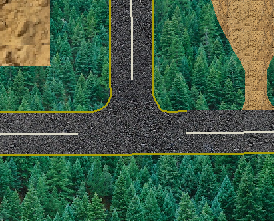
\includegraphics[width=0.5\textwidth]{intersection_original}
    \caption{A three way road intersection \label{fig:intersection_original} }
\end{figure}

The lanelets that describe the possible movements in this intersection are shown in figures \ref{fig:intersection_paths_group_1}, \ref{fig:intersection_paths_group_2} and \ref{fig:intersection_paths_group_3}.

\begin{figure}
    \centering
    \begin{subfigure}[b]{0.3\textwidth}
        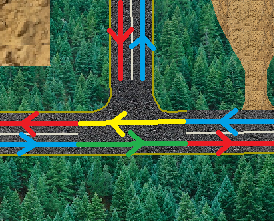
\includegraphics[width=\textwidth]{intersection_paths_group_1}
        \caption{Lanelets connecting left and right sections}
        \label{fig:intersection_paths_group_1}
    \end{subfigure}
    ~ %add desired spacing between images, e. g. ~, \quad, \qquad, \hfill etc. 
      %(or a blank line to force the subfigure onto a new line)
    \begin{subfigure}[b]{0.3\textwidth}
        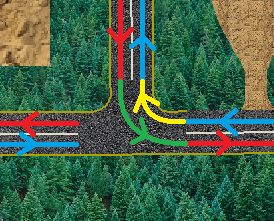
\includegraphics[width=\textwidth]{intersection_paths_group_2}
        \caption{Lanelets connecting top and right sections}
        \label{fig:intersection_paths_group_2}
    \end{subfigure}
    ~ %add desired spacing between images, e. g. ~, \quad, \qquad, \hfill etc. 
    %(or a blank line to force the subfigure onto a new line)
    \begin{subfigure}[b]{0.3\textwidth}
        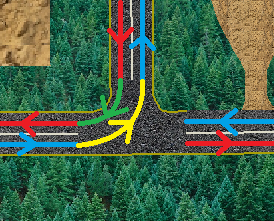
\includegraphics[width=\textwidth]{intersection_paths_group_3}
        \caption{Lanelets connecting top and left sections}
        \label{fig:intersection_paths_group_3}
    \end{subfigure}
    \caption{All the possible lanelets in a three way intersection}
\end{figure}

When all the lanelets of the intersection are put together, we create a functional piece of road network, with well defined car paths. Remember that a car can only travel between adjacent lanelets, and as such the road intersection does not allow for illegal movements, such as moving to a lane with a different direction.

Using this concept of lanelets and lanelet adjacency we can create a big variety of road networks with well defined rules of traffic flow. This is of extreme importance as we will see in the following sections.

MAYBE DO A LIST OF ADJACENCIES.

\subsubsection{Creating a Road Network}

Once the concepts of the road network are understood, we can start creating one. For this purpose we will use JOSM.

\paragraph{JOSM}

JOSM\cite{JOSM} is an OpenStreetMap editor. This editor provides a GUI to edit OpenStreetMap files/maps. We will make use of it to create a file that will define our road network. Figure \ref{fig:josm_sml} shows a snapshot of a JOSM program instance running.

\begin{figure}[h!]
    \centering
    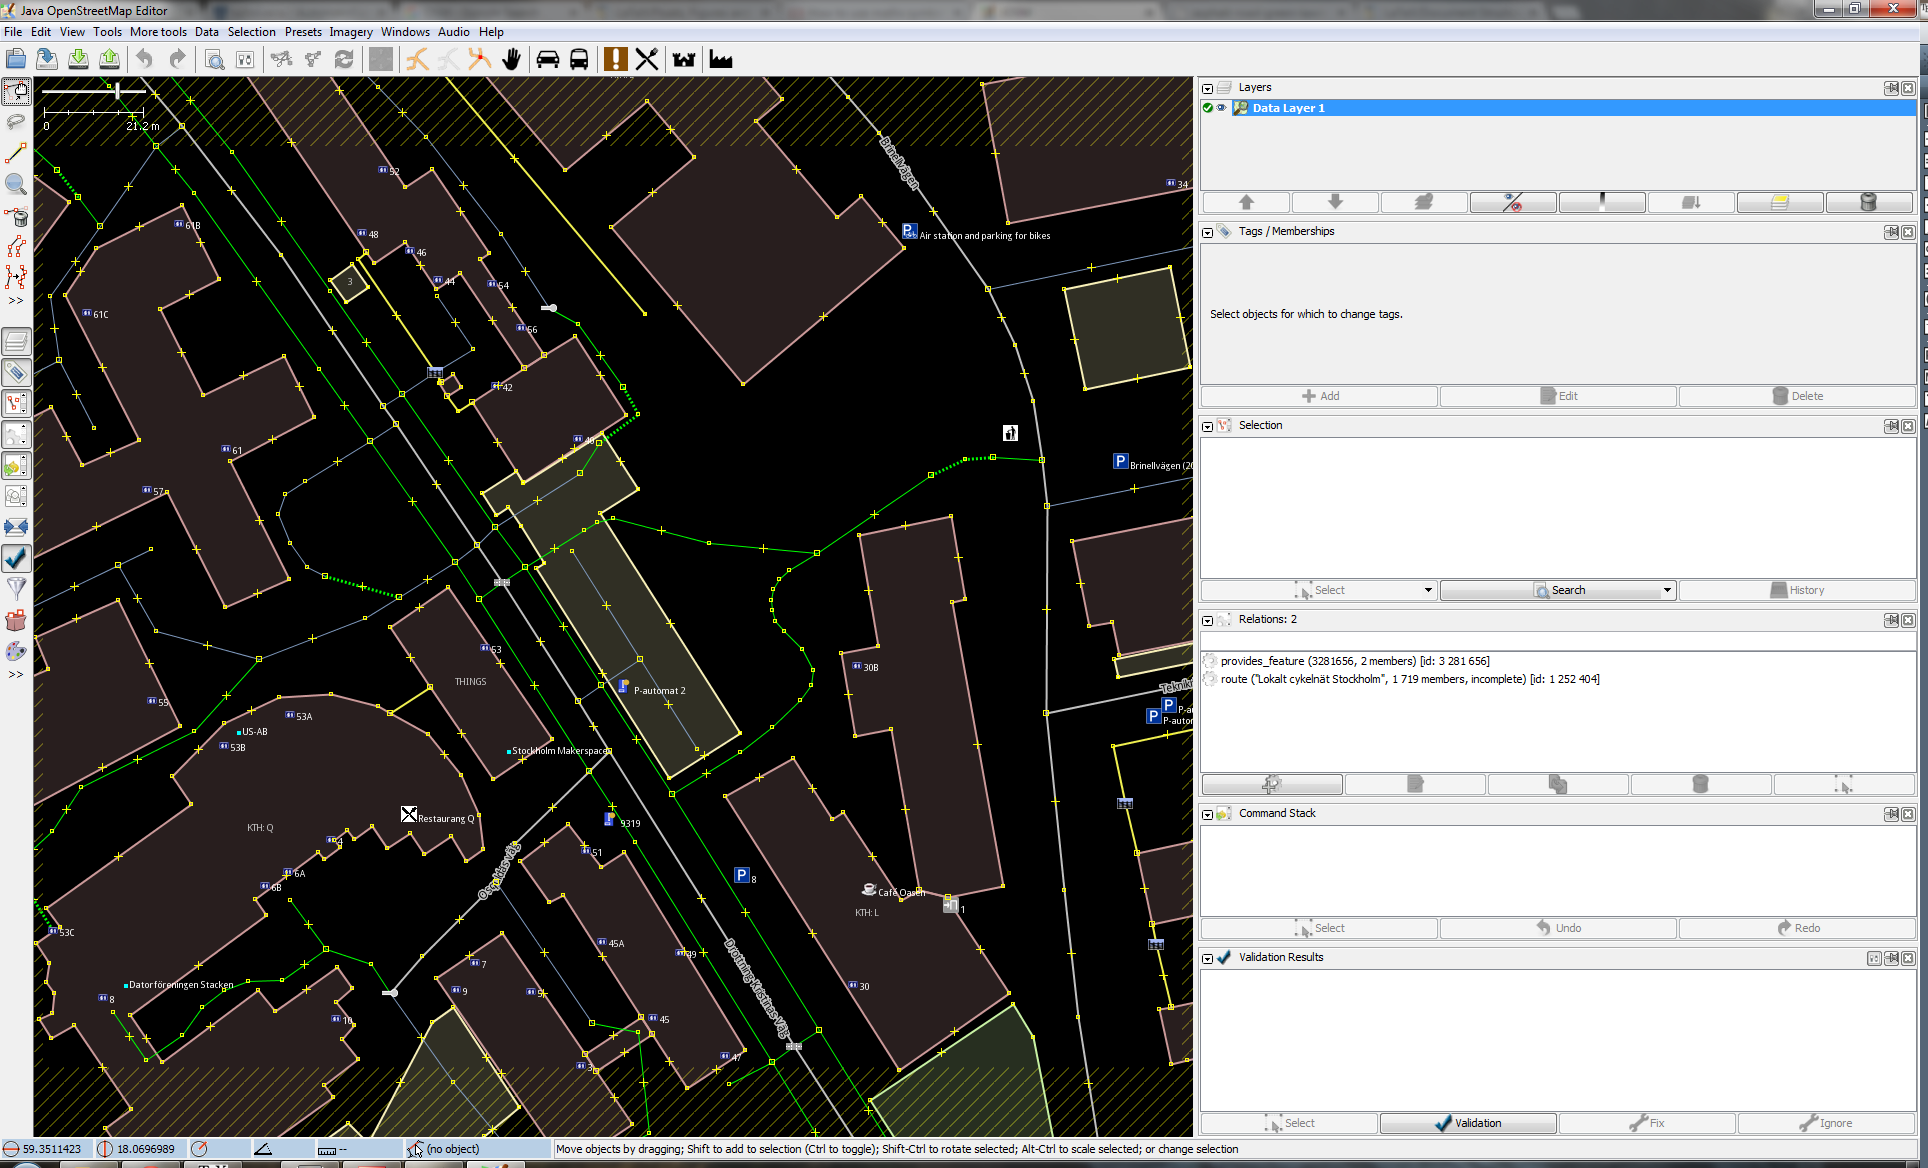
\includegraphics[width=0.75\textwidth]{JOSM_SML}
    \caption{An overview of the SML and surroudings OpenStreetMap map making use of JOSM \label{fig:josm_sml} }
\end{figure}

Here it will not be explained how to use JOSM, only how to build our road network making use of it. To understand how to work with JOSM refer to the guide available online.

\paragraph{Creating a Lanelet}

Before creating a lanelet, we need to create the ways corresponding to its left and right road markings. Lets start by creating the right road marking. To do so we simply create a way with the orientation that we wish our lanelet to have.

We could now use the same procedure to create the left road marking, however we are going to make use of the parallel tool to remove the ammount of work that placing the nodes requires. Besides being more efficient the parallel tool also guarantes that the new lane marking is parallel and in the same shape as the original lane marking, which should happen in every road.

An important detail is that the lanelet road marking ways need to have the same ammount of nodes, otherwise they cannot be processed by the SML World. The parallel tool complies with this requirement.

Once both ways are defined, we simply need to create our relation, which will represent a lanelet. Simply create a new relation, and the tag "type"="lanelet" and associate as members "right\_road\_marking" and "left\_road\_marking" the respective ways. The lanelet is now defined. 

\paragraph{Connecting Lanelets}

To connect lanelets, i.e., to make them adjacent we simply need to make sure that they have the same orientation, and that the first node of right way in one of the lanelets corresponds to the last node in the other lanelet.


\paragraph{Saving the Road Network File}

When the road network is complete, its corresponding information must be saved. JOSM allows saving the road network in several different file types, however we are interested in saving the file with the \textit{.xml} extension, meaning that we will have a simple to read XML file that can be easily used for future purposes.

If we wish to edit a previously save map, we simply need to open the corresponding \textit{.xml} file, edit it and save it again.

\paragraph{General Tips}

Using the parallel tool is often a good practice, due to the reasons already stated.

JOSM provides several tool, however that are some extra tools that can be added through the use of plugins. One of these tools is Circle Arc, which allows the user to draw circle arcs with relative ease.


\paragraph{List of Existing Road Networks OSM Files}

Some Road Networks were already made for previous usages. Their filenames and an explanation of their purposes will be given here.

\begin{description}

\item[HighwaySML.xml] This is the road network of a circular Highway with three lanes, all in the counter clockwise direction. This road network was used by the Summer Students of 2015, and it served to show possible solutions to the GCDC scenarios of platoons merging and emergency vehicle. The highway dimensions were fitted so that they allow for real live demonstrations using the scaled trucks. This road network can be altered to larger dimensions for simulation purposes.
\item[MiningEnvironmentSML.xml] This defined the road network used in the May 2015 IQMatic demonstration at Scania. It is composed of several roads and intersections, and it special environments for the scaled trucks to perform Autonomous Driving manoeuvres, like reverse driving and path planning. This map is not supported by the current SML World version, but can be useful in the creation process of new maps.
\item[SodertaljeResidentialArea.xml] This road network was based on a real residential road network. Defining road networks based on real existing ones can be useful to show and evaluate the performance of the autonomous driving system in realistic scenarios. This map is not supported by the current SML World version.
\item[RoadTemplates.xml] This file contains some useful and complex road network elements, like three and four way intersections. They can be easily copied for the creation of new maps.
\end{description}




\subsection{The Road Module}
\label{sec:roadmodule}

The Road Module is the name given to the Python class present in the SML World that is responsible for all the functionalities related to the road network. Its functionalities can be divided into two broad scopes, the computation of car trajectories and the visualisation of the environment.

In this section, we will give an overview of the functionalities that the Road Module provides, and an explanation of it's internal algorithms, when necessary.

\subsubsection{Processing the Road Network Map}

The first task of the Road Module, is to process and make sense of the Road Network Map. To do so, the constructor of the class is provided with the \textit{.xml} file containing this information.

The constructor will parse the \textit{.xml}, and the class will store dictionaries for the existing nodes, ways and lanelets in said file. Additionally a dictionary storing all the found tags, and corresponding nodes, is also created.

\paragraph{Converting from GPS to Meters}

As stated previously every OSM Node has an associated GPS latitude and longitude. For our purposes, we wish to have a simpler representation of the spatial location of the nodes, such as a Cartesian coordinate system in meters.

To do so we make use of the Python package \textbf{utm} (https://pypi.python.org/pypi/utm). This package allows us to make a conversion from GPS coordinates to a Cartesian referential as defined by the UTM convention. Once we have these new coordinates we will apply a translation transform so that they will be defined in a more convenient referential.

By default this new referential is located in the center of all the OSM Nodes. This center is computed easily by averaging the position of all the nodes. Once we know this center, we just need to subtract it from the coordinates of every single node, we will then have all of the node coordinates in the referential located in the center of all the nodes.

Another possibility is to define an Origin Node on which the referential will be located. To do so, when creating the \textit{.xml} file, one just need to and a node with the tag "origin"="true". If the Road Module detects that such a node is present in the file, it will simply subtract this node's Cartesian coordinates to all of the other nodes' coordinates, effectively making them be referenced on a referential located at the origin node.

\paragraph{Computing Lanelet Adjacencies}

One of the most important parts of the road network is the adjacency between the lanelets, for it defines the possible ways that cars can drive in them.

To fully describe the adjacencies between lanelets, we will make use of an Adjacency Matrix. An adjacency matrix A, is a square matrix with $n \times n$ elements, where $n$ is the number of lanelets in the road network.

\[
A_{n,n} = 
 \begin{pmatrix}
  a_{1,1} & a_{1,2} & \cdots & a_{1,n} \\
  a_{2,1} & a_{2,2} & \cdots & a_{2,n} \\
  \vdots  & \vdots  & \ddots & \vdots  \\
  a_{n,1} & a_{n,2} & \cdots & a_{n,n} 
 \end{pmatrix}
\]
 
The entry $a_{i,j}$ in the matrix indicates the adjacency value between lanelet $i$ and lanelet $j$. If its is possible to go from lanelet $i$ and lanelet $j$, \textit{i.e.}, if it lanelet $i$ is adjacent to lanelet $j$, the value of $a_{i,j}$ will be equal to the length of lanelet $i$.

If the it is not possible to go from lanelet $i$ and lanelet $j$, the value of $a_{i,j}$ will be infinity, or an extremely large number (in the SML World implementation this value is $10^{10}$).

Notice that $a_{i,j}$ is not necessarily equal to $a_{j,i}$, as being able to go from lanelet $i$ to lanelet $j$, does not imply that it is possible to go from lanelet $j$ to lanelet $i$.

\subsubsection{Computing Car Paths}

Computing a car path is equivalent to finding a valid/feasible way of going from one point in the road network to another. To do so, we divide this process in several parts.

\paragraph{The Start and End Nodes of the Path}

The main inputs to the Path Finding algorithm are the Start Node and the End Node. The start and the end nodes define, respectively, where we wish our path to start, and where we want it to end.

Given the start node, the Road Module will find the lanelet (or lanelets) that have this node in as part of their right\_lane\_marking way. For now lets assume that only one lanelet contains this node. The same is done for the end node, and the lanelet containing it is found. We now have two lanelets that we will call $lanelet_{start}$ and $lanelet_{end}$, which contain the start and end node, respectively.

We now have a way to move from $lanelet_{start}$ to $lanelet_{end}$. The solution to this problem will be a path of lanelets, that will start in $lanelet_{start}$ and finish in $lanelet_{end}$, making only legal movements, \textit{i.e.}, transitions between adjacent lanelets.

\paragraph{The Dijkstra Algorithm}

We wish to go from the starting lanelet to the ending lanelet, making transitions only between lanelets that are adjacent. We also want to do it in the best way possible, \textit{i.e.}, shortest way possible. 

This problem can be easily solved using the well known Dijkstra Algorithm. The Dijkstra algorithm is able to find the shortest path between nodes in a graph. We can view our road network as a graph of lanelets, in fact, the Lanelet Adjacency Matrix, perfectly defines a graph, where the lanelets are the nodes of the graph, and the edges are defined by the weights given by the adjacency matrix elements. An element of the matrix with an infinite value is equivalent to a non-existing edge.

This means, that having $lanelet_{start}$, $lanelet_{end}$, and the lanelet adjacency matrix, we can run the Dijkstra algorithm, and find the shortest path of lanelets between $lanelet_{start}$ and $lanelet_{end}$.

\paragraph{Generating the Path}

Assume now, that after our Dijkstra algorithm, we found a solution path $ [lanelet_{start},\allowbreak lanelet_{a},\allowbreak lanelet_{b},\allowbreak lanelet_{c},\allowbreak lanelet_{end}]$. We now wish to get the $(x,y)$ path corresponding to this lanelet path. 

The $(x,y)$ path of a lanelet, which is the set of points centred between the left\_lane\_marking and right\_lane\_marking, where each point is equally distant to the next and previous points.

We compute the $(x,y)$ path for each lanelet in the lanelet path, stitch them together, forming an $(x,y)$ from $lanelet_{start}$ to $lanelet_{end}$ that complies with the rules of the road network (as defined in the lanelet adjacency matrix).

This path still needs a final modification, however. The path is made up of the full $(x,y)$ paths of each lanelet, including the $lanelet_{start}$ and $lanelet_{end}$, however we might not need the full path of the $lanelet_{start}$ and $lanelet_{end}$. Take for example the case where the prvided ending node is located somewhere in the middle of $lanelet_{end}$. In this case we will not want the full $(x,y)$ path of the lanelet, but only the section that starts at the beginning of the lanelet, and ends close to he ending node. The same principle applies to the $(x,y)$ path of $lanelet_{start}$, however resulting path will begin at the starting node and continue until the end of the lanelet. We call this procedure, cropping the trajectory.

\paragraph{The "Circular" Dijkstra Algorithm}

The "Circular" Dijkstra algorithm is a special situation of the Dijkstra algorithm, in which we wish to find the shortest way from a node to itself, whilst assuming that nodes cannot connect to themselves. The importance of this algorithm for the SML World, has to do with generating paths that loop, thus resulting in motions that can run forever.

The original previous formulation of the Dijkstra algorithm does not allow us to solve this problem, however a simple reformulation can be done, that will allow us to find the shortest path from a node to itself.

To solve this problem we will need to create a new graph, that will be equivalent to the original graph, but that will allow us to solve the problem. Given that we want to find the shortest path from $node_i$ to itself, we will have to replace $node_i$ by nodes $node_i^{start}$ and $node_i^{end}$. $node_i^{start}$ will have all of the outgoing edges of $node_i$, and $node_i^{end}$ will have an of the incoming edges of $node_i$. 

Once this new graph is defined we can simply run a Dijkstra algorithm to find the shortest path between $node_i^{start}$ and $node_i^{end}$, and this will be equivalent to the shortest path from $node_i$ to itself.

\subsubsection{Environment Visualisation}

Besides defining how the road network behaves, the Road Module is also responsible for how the environment looks like. This is an important task as the visualisation of the environment plays a big role in the SML World.

Generating and visualising the environment requires the use of the graphical library pygame. More information about pygame can be found in their website \cite{pygame}.

\paragraph{Drawing Patterns}

The first step consists in generating the environment background. For this purpose we start by repeating the pattern image that we wish to fill the background with. Usually we use a forest pattern as can be seen in figure \ref{fig:visualisation_background}. The forest pattern is simply applied through the whole image, as it is a background pattern. One can choose different any possible background by selecting the appropriate image pattern.

\begin{figure}[h!]
  \centering
    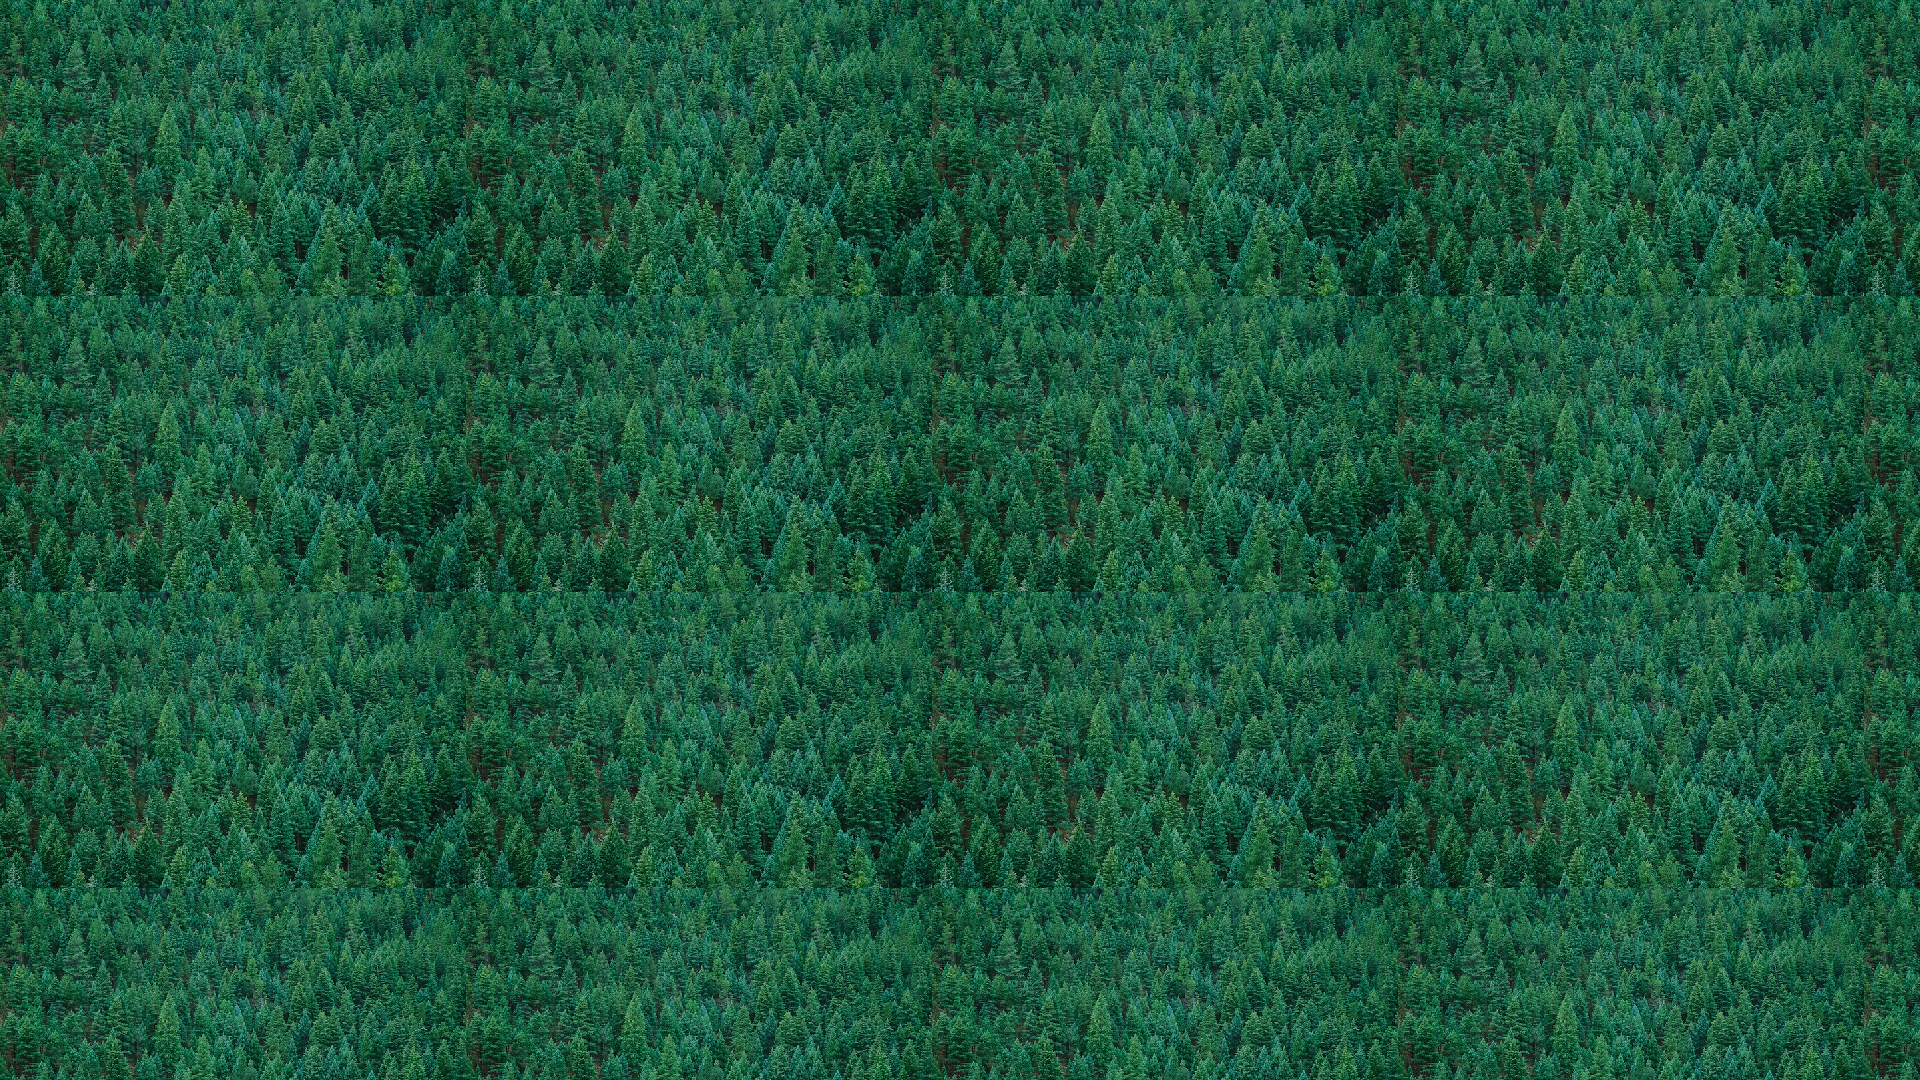
\includegraphics[width=0.95\textwidth]{visualisation_background}
    \caption{An environment with a forest pattern as background \label{fig:visualisation_background} }
\end{figure}

Once the background is drawn, we will overlay it with the roads. The roads are simply drawn by repeating a road pattern in the pixels corresponding to lanelets. First we find the regions of the lanelets, also called a mask. This mask tells us all the pixels that correspond to lanelets. Once we know this mask, we know where the lanelets are. We use this information to repeat the road pattern in the regions where there are lanelets. The result is shown in figure \ref{fig:visualisation_background_and_roads}. We can choose different looks for the roads by simply selecting the appropriate pattern image. 

\begin{figure}[h!]
  \centering
    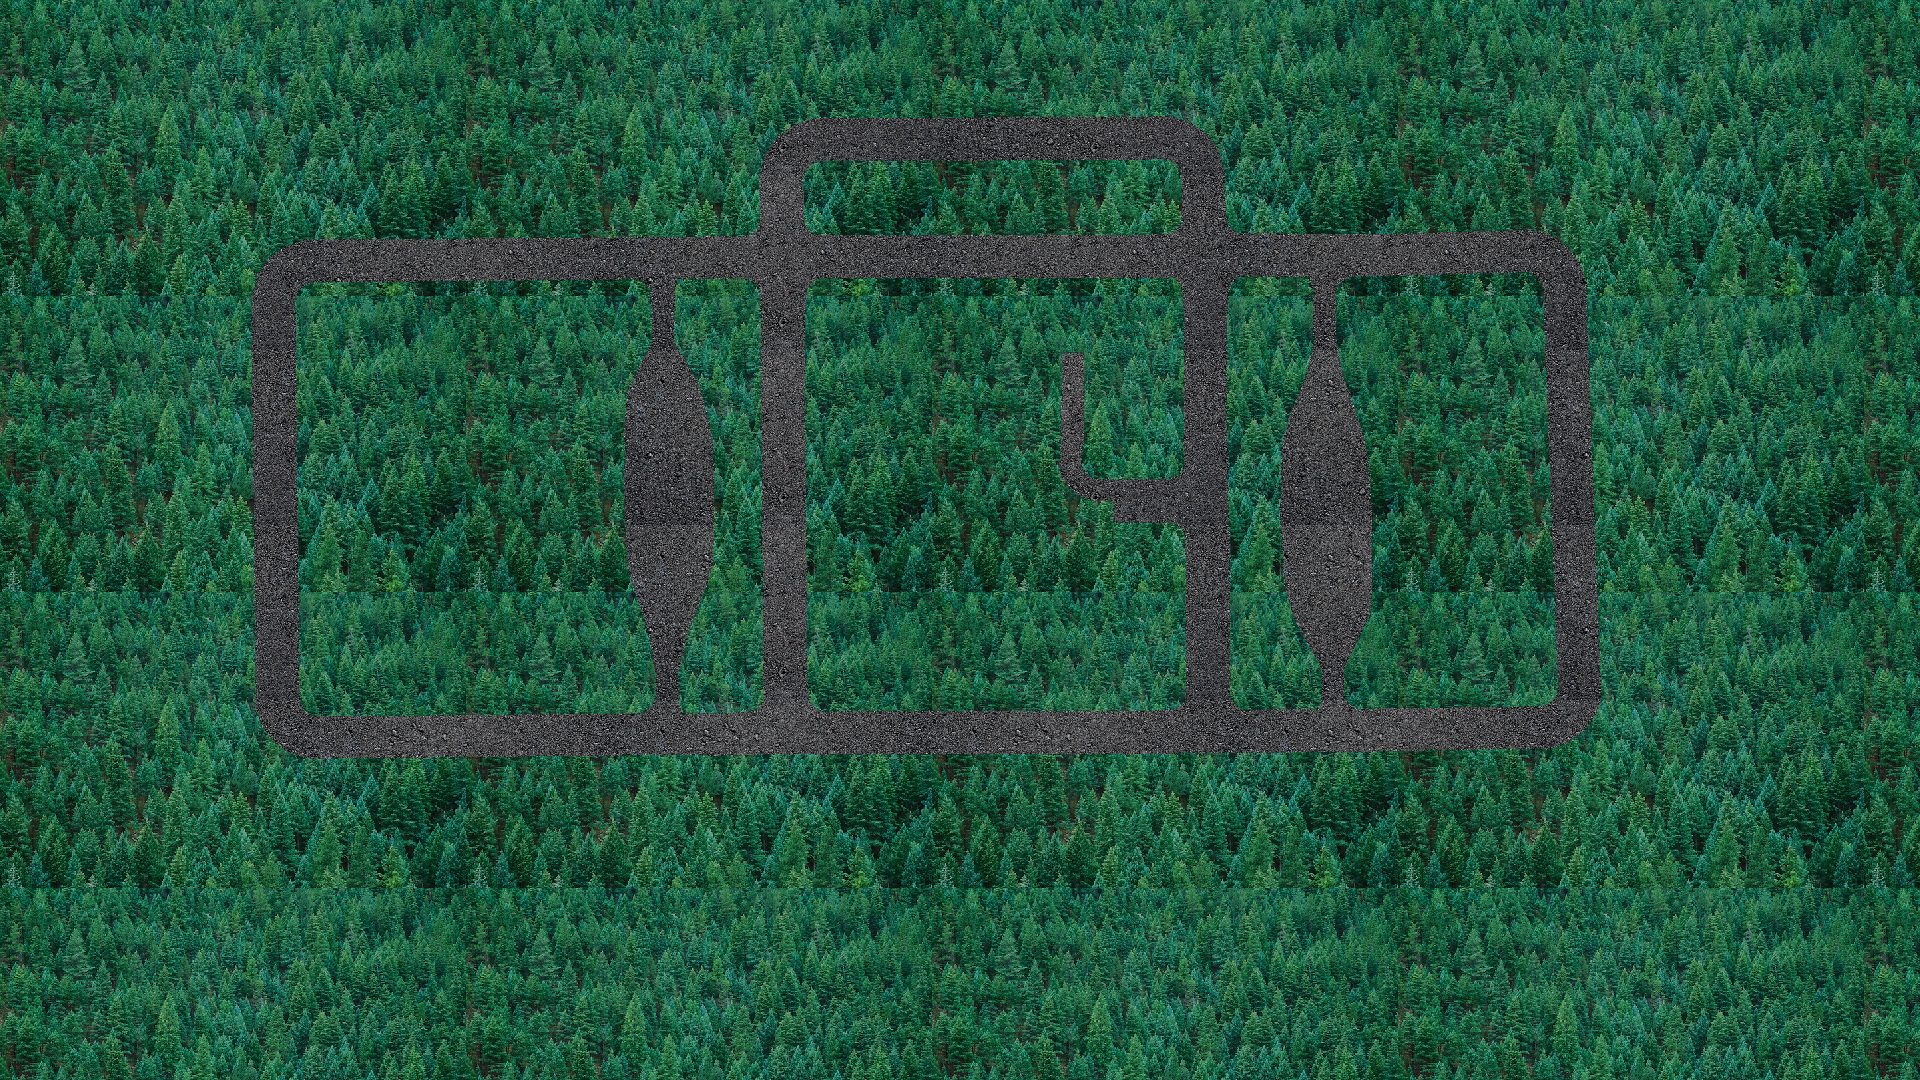
\includegraphics[width=0.95\textwidth]{visualisation_background_and_roads}
    \caption{An environment with a road pattern added \label{fig:visualisation_background_and_roads} }
\end{figure}

The environment visualisation can be made arbitrarily complex, if one uses this pattern repeat functionality to draw several different regions of different types. Figure \ref{fig:visualisation_background_with_several_patterns} shows an environment using five different patterns: forest, road, mud, iron and parking lot.

\begin{figure}[h!]
  \centering
    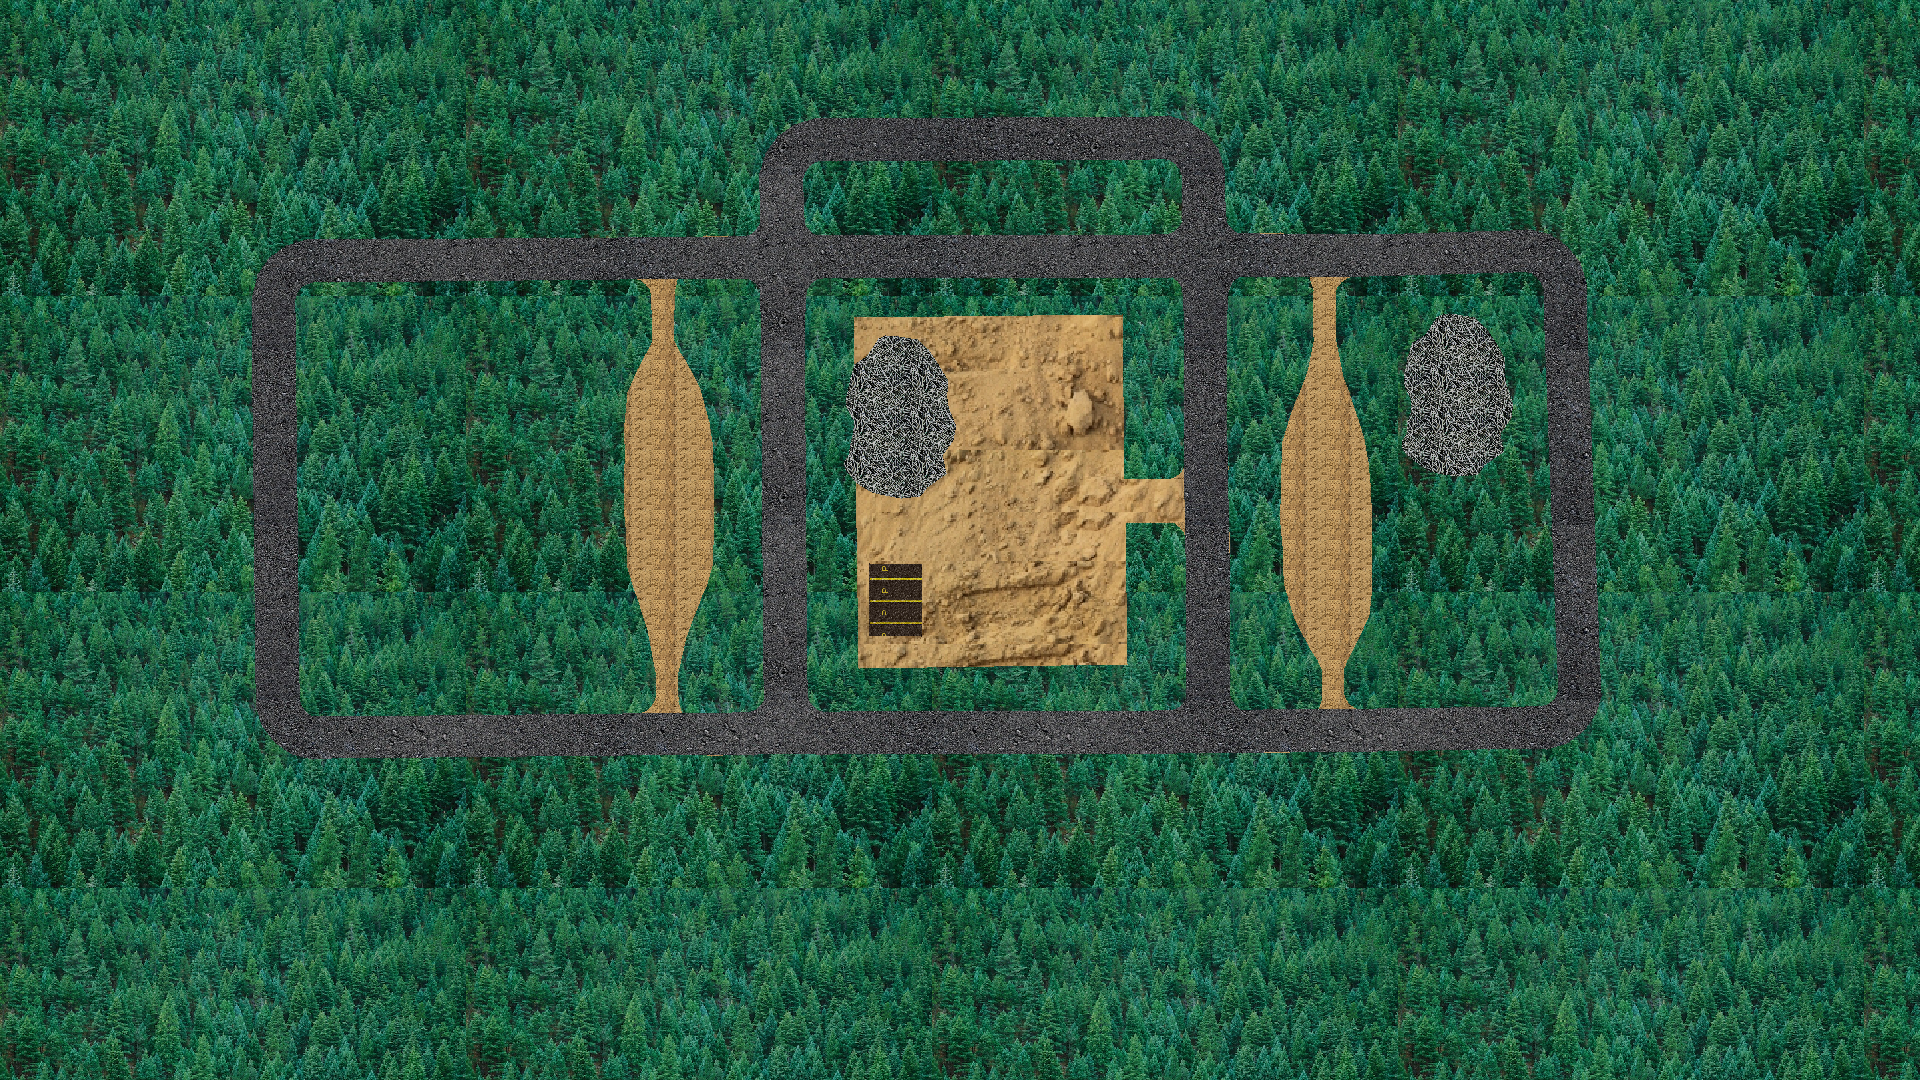
\includegraphics[width=0.95\textwidth]{visualisation_background_with_several_patterns}
    \caption{An environment using several patterns \label{fig:visualisation_background_with_several_patterns} }
\end{figure}

\paragraph{Drawing Lines}

Another important part of the environment visualisation is the ability to draw lines. Drawing lines comes in handy when drawing road markings. The road module is able to draw lines of different colors and different widths for ways that are present in the road network, this can be seen in figure \ref{fig:visualisation_background_and_roads_and_markings}. The road module will go over all of the ways present in the road network and it will draw lines on top of them if they have a specific tag. In case they have a tag "line\_type"="interior", they will be drawn as a white line, if the tag is "line\_type"="exterior" they will be drawn as yellow lines. If a way has no tag, a line is not drawn. 

\begin{figure}[h!]
  \centering
    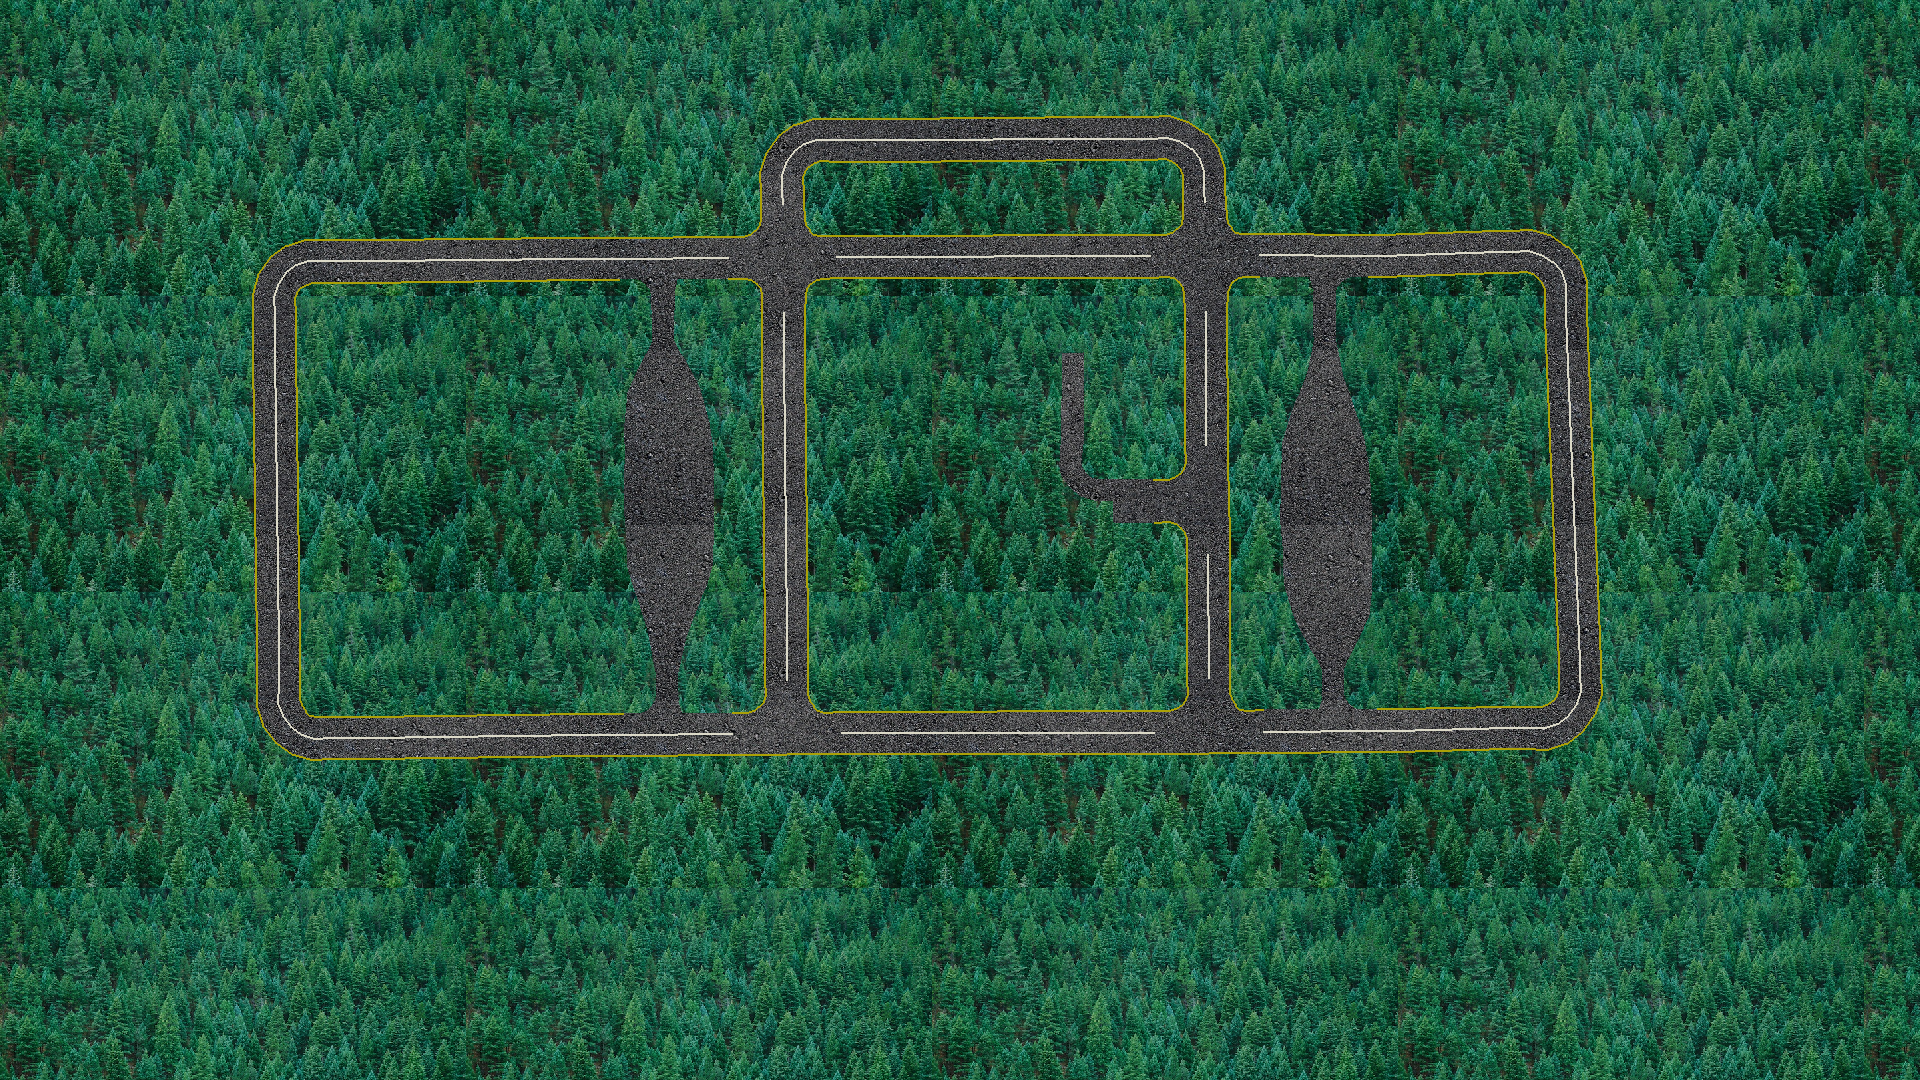
\includegraphics[width=0.95\textwidth]{visualisation_background_and_roads_and_markings}
    \caption{An environment with lines drawn \label{fig:visualisation_background_and_roads_and_markings} }
\end{figure}

\subsubsection{Using the Road Module}

Here we will briefly explain the main usages of the Road Module from a programming point of view. More detailed information is available in the source code.


\paragraph{RoadModule()}

road\_module = RoadModule(xml\_file\_location) Constructs an instance of the class \texttt{RoadModule}. The constructor requires that the location of the \textit{.xml} defining the road network is given.

\paragraph{SetImageProperties()}

SetImageProperties sets the properties of the image that will correspond to the environment. As arguments ImageWidth and ImageHeight correspond to the desired image width and height in pixels. PixelPerMeter will define how many pixels correspond to a meter in the map. Decreasing the value of PixelPerMeter will make the image correspond to a larger environment area.

\paragraph{GetEnvironmentImage()}

GetEnvironmentImage generates and returns the image of the enviroment. The arguments required are the same as the ones in SetImageProperties. This method returns a pygame Surface corresponding to the environment image.

\paragraph{GetPathBetweenNodeIds()}

GetPathBetweenNodeIds returns an $(x,y)$ path between two nodes. The arguments are StartOsmNodeId and EndOsmNodeId, which correspond to the ids of the nodes we wish that define this path. The third argument is PointsPerMeter wich indicates how many path points will be generated for each meter of path.

\paragraph{GetPathBetweenNodeTags()}

Equivalent to GetPathBetweenNodeIds, however instead of having node ids as arguments, we have node tags. This allows for a simpler usage, as it is usually easier to know the tag of a node (it can be easily added on the road network \textit{.xml} file), than its id.

\paragraph{GetClosedPathFromNodeId()}

Returns the $(x,y)$ path that starting and ending on a given node. The arguments are OsmNodeId and PointsPerMeter. OsmNodeId corresponds to the id of the node we wish to have the circular path of. PointsPerMeter will define how many path points will be generated for each meter of path.

\paragraph{GetClosedPathFromNodeTag()}

Equivalent to GetClosedPathFromNodeId, however istead of providing a node id, the user provides a node tag.

\subsubsection{Deprecated Functionalities}




Talk about how to draw patterns given a way and a tag.




\graphicspath{ {SectionTheSimulationModule/Images/} }

\section{The Simulation Module}
\label{sec:the_simulation_module}

The Simulation Module implements one of the most fundamental tasks in the SML World, the Simulation of vehicles. It is, however, not limited to the simulation of the vehicle in itself, but also to the simulation of sensors that might be equipped in said vehicles.

In this the Simulation Module structure will be explained, as well as the simulation models used for the vehicles and for the vehicle sensors.

\subsection{The Simulation Module Class}

Remembering from the explanation given in \ref{subsubsec:simulation_module} (and additionally from figure \ref{fig:sml_world_structure_3}) we know that the Simulation Module will be running in an individual thread of execution in parallel with the SML World. It is however a part of the SML World, and it needs, by design, to interact with it.

The SimulationModule class, which implements the Simulator Module is defined in the file \texttt{SimulatorModule.py}. This class will have acess to the SML World, and it will interact heavily, reading and modifying, the vehicles stored in the Vehicles Dictionary.

\subsubsection{Constructor}

The constructor takes as arguments the SML World instance, and the desired simulation rate.

The SML World instance allows the Simulation Module class to have access to the SML World and its Vehicles Dictionary.

The second argument of the constructor, the desired simulation rate, defines the rate at which we wish the vehicles states and sensor readings to be updated (simulated). The Module will try to keep this rate as best as it can, however if it cannot keep up with this rate (due to low processing power for example), it will output warning messages to the terminal, letting the user know of this fact.

One can always reduce the desired rate of simulation in order to make sure that the Simulation Module can run at the desired rate. However the simulation quality decreases with the decrease of the simulation rate. By default the simulation rate is set to $50 Hz$.

The last step of the class constructor is creating the parallel thread of execution which will run the main loop.

\subsubsection{Main Loop}

The Main Loop of the class is defined in \texttt{thread\_loop}, and it is a fixed (given that there is enough processing power) rate loop that runs in parallel thread of execution while the SML World is running. This loop is responsible for calling the \texttt{simulate\_vehicles} and \texttt{simulate\_sensor\_readings} methods of the class.

\subsubsection{Vehicle Simulation}

The Vehicle Simulation is implemented by the \texttt{simulate\_vehicles} method, which will simply iterate over all the vehicles present in SML World's Vehicles Dictionary and update their states according to the simulation model used. The simulation model is defined by the Vehicle's Class method \texttt{vehicle\_state\_update}, and as such it is the task of the Vehicle Class to define the simulation model to be used. More details on the possible simulation models to use are provided in \ref{subsec:vehicle_models}.

The \texttt{simulate\_vehicles} method takes as argument \texttt{time\_to\_simulate} which corresponds to the amount, in seconds, of time that we wish to simulate. If the current vehicle states in the SML World correspond to time $t$, then the new updates states of said vehicles will correspond to time $t+\texttt{time\_to\_simulate}$.

The argument \texttt{time\_to\_simulate} is computed by the Main Loop (\texttt{thread\_loop}) and it will correspond to the time elapsed since the last call to \texttt{simulate\_vehicles} was made. This guarantees that even in situations where the desired simulation rate cannot be achieved, the simulation will compensate for it, and keep the vehicle states evolving in real time by simply simulate for a longer period of time. The inherent downside is that the simulation will inevitably lose quality. 


\subsubsection{Sensor Simulation}

The task of simulating the readings provided from the vehicle sensors is left to the \texttt{simulate\_sensor\_readings} method. Similarly to the \texttt{simulate\_vehicles} method, it will iterate over the vehicles present in the Bodies Dictionary, however instead of updating (altering) the vehicles' states it will change the vehicles' sensor readings. It does so by calling Vehicle's method \texttt{set\_sensor\_readings}.

This function does not have input arguments, but relies on the Vehicle Class' attributes to know which sensors to simulate. The boolean attributes \texttt{radar\_mode}, \texttt{velodyne\_mode} define if a Vehicle is equipped with Radar and/or Velodyne sensors, respectively. There is also the possibility to simulate a perfect sensor that is aware of every other vehicle in the SML World, and it can be turned on through the attribute \texttt{omniscient\_mode}. The implementation details of each sensor are given in \ref{subsec:sensor_models}.

\subsection{Vehicle Models}
\label{subsec:vehicle_models}

The vehicle models define how the vehicle states will evolve when being simulated. They can be made arbitrarily complex, in order to achieve realistic behaviour, however such models might be computationally expensive and slow. The choosing of an appropriate vehicle model is then a trade-off between realistic behaviour and computational efficiency. The current model used for the \texttt{smartvehicle.py} Vehicle Class is the Acceleration based Unicycle Model explained in \ref{subsubsec:acceleration_based_unicycle_model}.

\subsubsection{Kinematic Unicycle Model}
\label{subsubsec:kinematic_unicycle_model}

One of the simplest models to simulate a car movement is the kinematic model for a simple car with the position, $(x,y)$, and orientation, $\theta$, states. Said car has as commands a steering angle, $\phi$ and a linear velocity $v$.

Knowing the current state and command inputs, we can compute the derivatives of the state as 

\[
\label{eq:kinematic_car_model}
\begin{array}{rcl}
\dot{x} & = & v \cos{\theta} \\
\dot{y} & = & v \sin{\theta} \\
\dot{\theta} & = & ( \nicefrac{v}{L} ) \tan{\phi} 
\end{array}
\]

Parameter $L$ corresponds to the distance between the front and rear axles of the car. Knowing the derivatives of the state we can compute the next state, $\Delta t$ seconds after the current state using the approximation

\[
\begin{array}{rcl} 
x_{t+\Delta t} & = & x + \dot{x} \times \Delta t \\
y_{t+\Delta t} & = & y + \dot{y} \times \Delta t \\
\theta_{t+\Delta t} & = & \theta + \dot{\theta} \times \Delta t \\
\end{array}
\]

Of course the bigger the $\Delta t$, the rougher the estimation. That is why one should have an high simulation rate, as $\Delta t$ is the inverse of the simulation rate $\Delta t = \nicefrac{1}{\texttt{simulation\_rate}}$.

\subsubsection{Acceleration based Unicycle Model}
\label{subsubsec:acceleration_based_unicycle_model}

The acceleration based unicycle model builds upon the kinematic unicycle model described before, however it now adds assumes that the linear velocity of the car is follows an acceleration model equation.

To implement such a model, the vehicle state has to now include the velocity states $(\dot{x},\dot{y})$, which are used to determine the instantaneous linear velocity $v=\sqrt{\dot{x}^2 + \dot{y}^2}$. Furthermore, instead of a velocity command input, we now have a throttle command input. The evolution of the $(x,y,\theta)$ states will still be described by equations \ref{eq:kinematic_car_model}, however the evolution of the linear car velocity $v$ is given by:

\[
\dot{v} = \frac{throttle - c\times v}{m}
\]

Where $throttle$ is the throttle produced by the car, $c$ is the air drag coefficient of the car, and $m$ its mass.

\subsection{Sensor Models}
\label{subsec:sensor_models}

Sensor models are used to determine what information a sensor can provide to a car given its current surroundings. The sensor models used here will assume that the sensor is capable of processing the information it gathers, and convert it to an understandable vehicle state given by $(x,y,\dot{x},\dot{y})$ and respective id.

The only difference between the sensors that will be described later is then related only to its region/area of sensing, that is, how far and wide can a sensor detect other vehicles.

By simulating the sensors in this way, we are jumping over one of the big problems of autonomous driving, the processing and understanding of data coming from sensors. This is not a problem however, since the current scope of the SML World does not focus on the area of Sensors and Data Fusion.

\subsubsection{Radar}

The Radar sensor will be able to detect vehicles that are in a cone shaped region situated in front of the ego vehicle. This region is defined by two attributes \texttt{radar\_angle} and \texttt{radar\_range}. The radar angle determines the field of sensing of radar, the larger it is the wider the sensing cone. The radar range in turn will determine how far can the radar sense, this can be thought of as the height of the cone. Figure \ref{fig:radar_sensing_area} shows the sensing cone of a vehicle's radar, and how these attributes shape the sensing area of the radar.

\begin{figure}[h!]
  \centering
    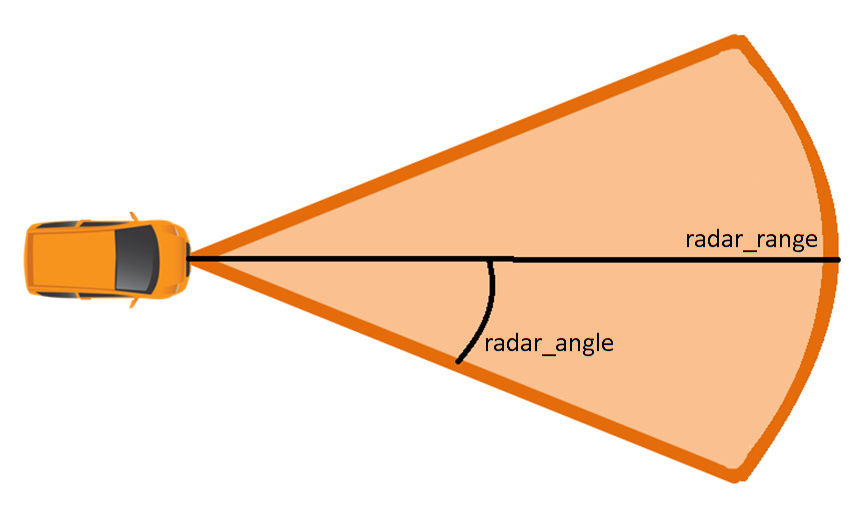
\includegraphics[width=0.9\textwidth]{radar_markings_quantities}
    \caption{Representation of the radar sensing area \label{fig:radar_sensing_area} }
\end{figure}

This sensor can be toggled on or off using the boolean attribute \texttt{radar\_mode}. The sensor provides readings for each vehicle in the sensing area in the form of $(id, x, y, \dot{x}, \dot{y})$.


\subsubsection{Velodyne}

The Velodyne sensor is a sensor used by KTH's Research Concept Vehicle which is able to sense objects in a 360 degree area. To completely define this sensor we just need to set the value of  \texttt{velodyne\_range} which determines the radius of the sensing circle of the Velodyne. Figure \ref{fig:velodyne_sensing_area} shows the sensing area of this sensor.

\begin{figure}[h!]
  \centering
    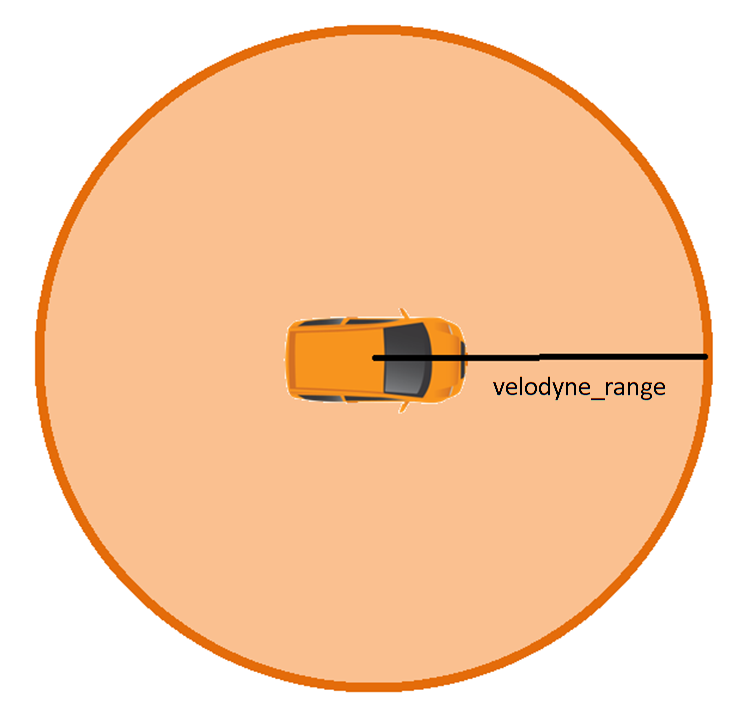
\includegraphics[width=0.75\textwidth]{velodyne_markings_quantities}
    \caption{Representation of the velodyne sensing area \label{fig:velodyne_sensing_area} }
\end{figure}

The Velodyne sensor can be toggled on or off using the boolean attribute \texttt{velodyne\_mode}. The sensor provides readings for each vehicle in the sensing area in the form of $(id, x, y, \dot{x}, \dot{y})$.

\subsubsection{Omniscience}

A perfect sensor can also be simulated by toggling the attribute \texttt{omniscient\_mode}. If activated this sensor will get the readings of every vehicle present in the SML World, no matter how far they might be. The sensor will thus provide readings for all the vehicle in the SML World in the form of $(id, x, y, \dot{x}, \dot{y})$.





\section{The V2V Module}
\label{sec:the_v2v_module}

The V2V Module is responsible for simulating message transmissions between vehicles in the SML World. Autonomous vehicles might require an exchange of information between them, which can be achieved in several ways. The V2V Module, will try to simulate the possibilities and constraints of Network and Wi-Fi based communications between vehicles. While the Network communications allow for vehicles to speak with each other, no matter how distant they are, Wi-Fi allows only for communications over a short range. However Wi-Fi performs as a much faster rate, being able to transmit more information and with a lower delay than the Network. Details about each method's implementation will be given in the following pages.

\subsection{The V2V Module Class}

The V2V Module Class gives the SML World the possibility of simply instantiating an object of the class that will initialize itself and start running, in parallel, an execution loop in a individual thread of execution.

This object will have acess to the SML World, and will interact, reading and modifying, with the Objects Dictionary. This is done in order to update the messages that each vehicle is sending or receiving.

At the moment, the V2V Module Class is assuming that the only vehicles of the type SmartVehicle (\texttt{smartvehicle.py}) are able to exchange messages. They do so by making use of incoming and outgoing message buffers, for the Network and Wi-Fi channels. These channels are implemented as attributes of the SmartVehicle class and can be interfaced with through the SmartVehicle methods \texttt{set\_network\_input\_messages}, \texttt{get\_network\_output\_messages}, \texttt{set\_wifi\_input\_messages} and \texttt{get\_wifi\_output\_messages}.

The messages can be implement as any object desired, examples of possible objects are strings, dictionaries or a user-made custom class. It is the task of the SmartVehicle to know how to encode and decode such messages.

\subsubsection{Constructor}

To instantiate the \texttt{SimulatorModule} class, a \texttt{loop\_rate} has to be provided, this will define the rate of the main loop that will run forever in it's own thread. This main loop is the one that simulates the communications of the SML World. More detail about the loop will be given in the following section. 

The Constructor also gets a reference to the SML World, so that it can have access to it, and most importantly, interact with the Bodies Dictionary. 

In the initialization process the attributes \texttt{v2v\_network\_rate} and \texttt{v2v\_wifi\_rate} are also defined. These determine the frequency at which messages can be exchanged by the Network and Wi-Fi channels.

\subsubsection{Main Loop}

The Main Loop will be running until the SML World is terminated. Its main function is to call the methods that simulate the exchange of communications between vehicles. The two methods implementing the communication exchanges are \texttt{network\_step} and \texttt{wifi\_step}.

The Main Loop will be in charge of calling such methods with the correct rate, as given by attributes \texttt{v2v\_network\_rate} and \texttt{v2v\_wifi\_rate}. If the Main Loop cannot comply with its desired rate of \texttt{loop\_rate}, due to intensive processing for example, it will print warnings to the terminal.

\subsection{Network Communication}

The Network Communications are implemented by the method \texttt{network\_step}. This method will iterate over all the vehicles in the Vehicles Dictionary and collect their output messages, by polling the Vehicle's output network buffer through the method \texttt{get\_network\_output\_messages}.

Once all the messages from all the vehicles are collected, we once again iterate over all of the vehicles and set them as inputs of every vehicle using the Vehicle method \texttt{set\_network\_input\_messages}. Messages sent by a specific vehicle are not returned to that same vehicle.

\subsection{Wi-Fi Communication}

The Wi-Fi Communications introduce an extra difficulty, which is related to the range of communications. Vehicles using Wi-Fi can only communicate with vehicles within a range of \texttt{v2v\_wifi\_range} meters.

The following algorithm is used to simulate the Wi-Fi communications:

\begin{algorithm}[H]

 \For{EgoVehicle in Bodies Dictionary}{
 
	InputMessages = Empty List 
 
 	\For{OtherVehicle in Bodies Dictionary except EgoVehicle}{
 	
		\If{distance between EgoVehicle and OtherVehicle \textless v2v\_wifi\_range}{
			Add OtherVehicle's \texttt{get\_wifi\_output\_messages} to InputMessages List
		}
	 	
 	}
 	
	EgoVehicle's \texttt{set\_wifi\_input\_messages} = InputMessages
 	
 }
 \caption{Wifi Message Exchange Algorithm}
\end{algorithm}

The above algorithm, does not represent the actual implementation details, but it does represent the concept idea that is implemented.


\section{The Smart Vehicle}
\label{sec:the_smart_vehicle}


\section{The Visualisation Module}
\label{sec:the_visualisation_module}

The VisualisationModule class is responsible for showing the current state of the environment, and the vehicles in it, in an appealing and realistic fashion.

To do so, the Visualisation Module opens up a Visualisation Window, where the user can get a bird's eye view of the environment, that is updated in real time. This module relies heavily on Python's graphical library pygame.

The Visualisation Module interfaces with the SML World through the use of UDP communications, implemented in the auxiliary classes VisualisationModuleSender and VisualisationModuleReceiver.

\subsection{The Visualisation Module}

The objective of the Visualisation Module is to show to the user, the environment in a Visualisation Window. Unlike other Modules, the Visualisation Module runs independently (\textit{i.e.}, in a completely independent thread, see \ref{visualisation_module:threading_restrictions}) from the SML World. Image \ref{fig:visualisation_module_diagram} shows a diagram representing its structure.

\begin{figure}[h!]
  \centering
    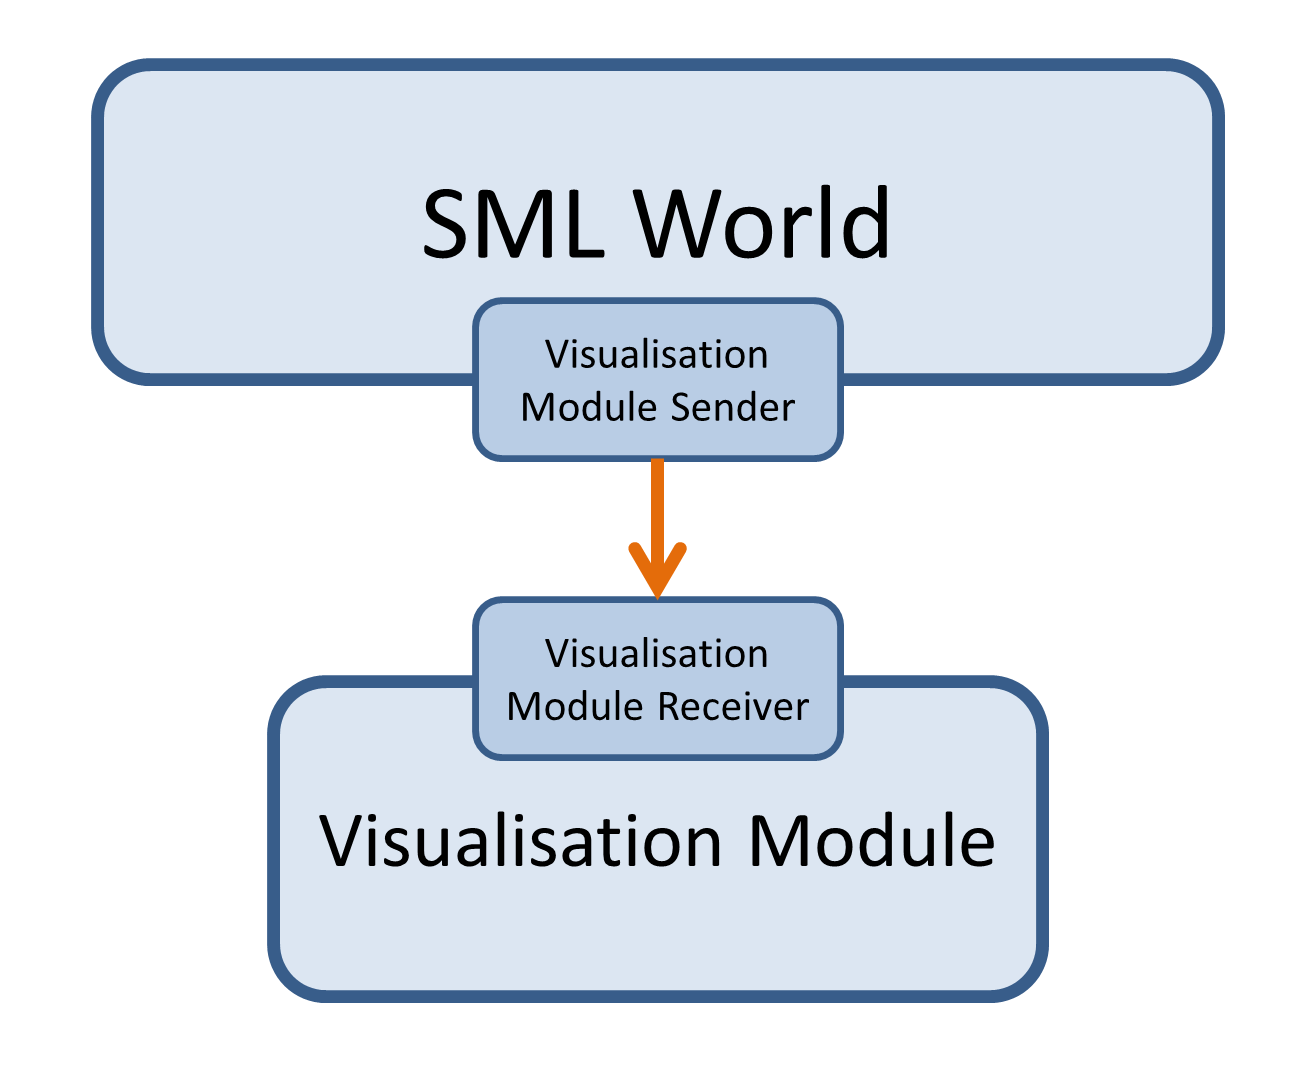
\includegraphics[width=0.6\textwidth]{visualisation_module_diagram}
    \caption{Diagram of the Visualisation Module interfacing with the SML World \label{fig:visualisation_module_diagram} }
\end{figure}

The SML World and Visualisation Module interface with each other using the auxiliary classes VisualisationModuleSender and VisualisationModuleReceiver. These classes establish a one-way UDP communication from the SML World to the Visualisation Module. The information transmitted over this communication link consists of the current vehicle states in the SML World.

\subsubsection{Loading the Environment Information}

The first step of the Visualisation Module is to load the environment information. This corresponds to the image depicting the environment, and the properties of this image.

To do so, the class constructor receives an argument \texttt{map\_filename}. This corresponds to a string with the location and name of the image to be loaded. This string must not have the extension of the image in it, since we will simply use the name of the image to fetch, both the image, and the metadata associated with the image. The image is simply obtained by appending the bitmap image extension (\texttt{map\_filename + .bmp}). The metadata of the image can be found as \texttt{map\_filename + .meta}.

The metadata file contains information about the image size, width and height, and the ration of pixels per meter. This information is necessary in order to know where in the image the vehicles should be drawn, given their Cartesian coordinates.

\subsubsection{From Meters To Pixel}

An important step in the Visualisation Tool, is to know where to draw the vehicles. Or in more simple terms, if I have a vehicle at cartesian coordinates $(x, y)$, what is the corresponding pixel position? To do so we need to define our meters to pixel converter function.

By default, all of the generated images, have the cartesian coordinate system originating at the center of the image. This means, that an object in coordinates $(x = 0, y = 0)$, will have its corresponding pixel be $(p_x = c_x, p_y = c_y)$, where $c_x$ and $c_y$ are the halves of the image width and image height respectively.

If an object is located one meter to the right of the coordinate origin, $(x = 1, y = 0)$, we now need to add the corresponding offset in pixels to find the respective pixel. This is achieved, very simply, by multiplying by the \texttt{pixel\_per\_meter} ratio, that converts meters in the SML World to pixels. The corresponding pixel to $(x = 1, y = 0)$ would be $(p_x = c_x + pixel\_per\_meter, p_y = c_y)$.

Applying the same idea, to offsets in the $y$ dimensions, we arrive at the general meters to pixel converter function: $(p_x, p_y) = (c_x + pixel\_per\_meter\times x, c_y + pixel\_per\_meter\times y)$.

An important note must be made, since the coordinate sytem of the Pygame image is defined in a different way (SEE FIGURE), the actual converting function is given by $(p_x, p_y) = (c_x + pixel\_per\_meter\times x, c_y - pixel\_per\_meter\times y)$.


\subsubsection{Adjusting to Screen Size}

The Visualisation Module user can determine the preferred pixel width and height for the visualisation window. This allows the Visualisation Module to run in both small and big screens.

In order to achieve this the user can give the arguments \texttt{window\_width} and \texttt{window\_height} to the class constructor. The class will then compute the necessary image transforms in order to convert the source image, into an image with the desired dimensions of the visualisation window.


\subsubsection{Adjusting to SML's Ceiling Projector}

Another constructor argument of the class is the boolean \texttt{ground\_projection}. When set to True we will assume that the user wishes the visualisation window to be displayed on SML's ground projector.

In order to correctly display the image on the ground projector, some extra steps need to be taken. First we measured the dimensions, in meters, of the SML Projector ground display. This gives us the area/positions, in meters, where the display will be on the ground. Knowing that the SML is a 1/32 scale model (mostly because of the trucks in use), we can multiply the original projector dimensions by 32, and we will obtain the Simulation Dimensions of the projector, that is, the dimensions, in Simulator meters, that the projector corresponds to.

Knowing these dimensions, we get the corresponding section of the original image, which is then scaled to the Visualisation Window dimensions. The visualisation windo dimensions here are simply the size of the projector screen, which is usually 1400*1050.

An extra detail, is that the visualisation window will not have a bordering frame, this can be achieved by adding the flag \texttt{pygame.NOFRAME}, to the \texttt{pygame.display.set\_mode} function.

\subsubsection{Creating Vehicle Images}
\label{visualisation_module:creating_vehicle_images}
Before drawing vehicles on the SML World, one needs to get their corresponding images. The car images are stored in the \texttt{resources} folder. These images need to follow a set of restrictions to make sure that they are correctly used by the Visualisation Module.

Let's imagine we want to use figure \ref{fig:visualisation_module:car_image} to represent our car.

\begin{figure}[h!]
  \centering
    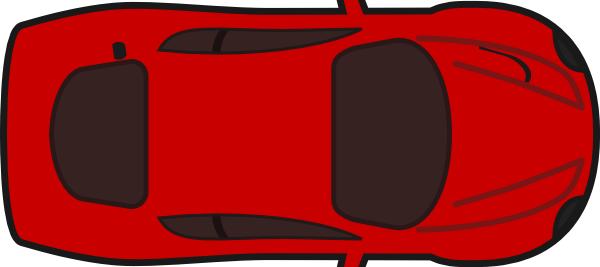
\includegraphics[width=0.6\textwidth]{car_image}
    \caption{An image of a car \label{fig:visualisation_module:car_image} }
\end{figure}

The first thing we need to make sure of is that the image has equal pixel to meter ratio in both its horizontal and vertical components. That is, if the car has a width of 2 meters and the image an height of 100 pixels (remember that the image heigth corresponds to the car width), then if the car length is $x$ meters, the image width should be equal to $x \times \frac{100}{2}$.

This leaves us with the image shown in figure \ref{fig:visualisation_module:car_image_explained_1}. The blue rectangle represents the limits of the image, and is simply shown here for an easier understanding, it is not part of the image. Notice that the image is limited to include only the car, and not any additional empty space.

\begin{figure}[h!]
  \centering
    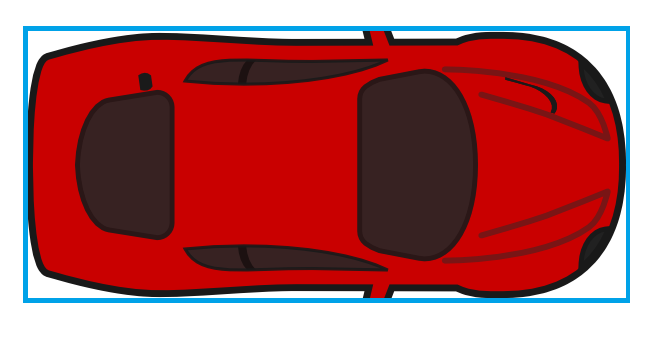
\includegraphics[width=0.6\textwidth]{car_image_explained_1}
    \caption{The car image cropped to the car region \label{fig:visualisation_module:car_image_explained_1} }
\end{figure}

The next step consists in translating the car image such that the center of rotation of the car (usually located in the middle of the rear axle) corresponds to the center of the image. The resulting image would look like the one in figure \ref{fig:visualisation_module:car_image_explained_2}.

\begin{figure}[h!]
  \centering
    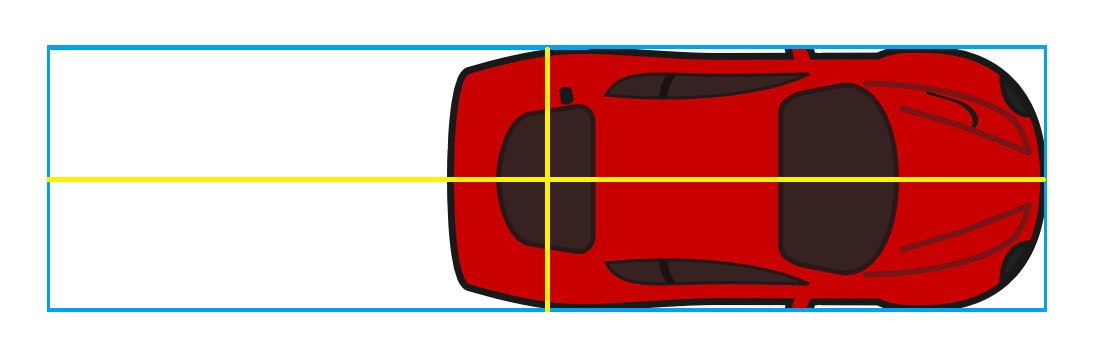
\includegraphics[width=0.9\textwidth]{car_image_explained_2}
    \caption{The car image offsetting the rear axle middle to the center of the image\label{fig:visualisation_module:car_image_explained_2} }
\end{figure}

The yellow lines correspond to the center of the image, like the blue rectangle they are only show for understanding purposes, they are not part of the image. The car rear axle is now located exactly in the center of the image. We make this requirement, since pygame is able to easily rotate images around their center, and as such, if we want to rotate a car, we can simply rotate its image, given that the car rear axle is located in the center of the image.

The final step in the image creation process consists in making it transparent in the pixel regions that do not correspond to the car. Image \ref{fig:visualisation_module:car_image_explained_3}, shows the final car image, with the transparent areas colored in grey. Once again, the grey region is not grey in the car image, but instead is transparent.

Transparency in images can be achieved only by certain image file formats, being \texttt{png} one of them. For creation of these images one can use many image editing programs, the author recommends the free program GIMP \cite{GIMP}.

\begin{figure}[h!]
  \centering
    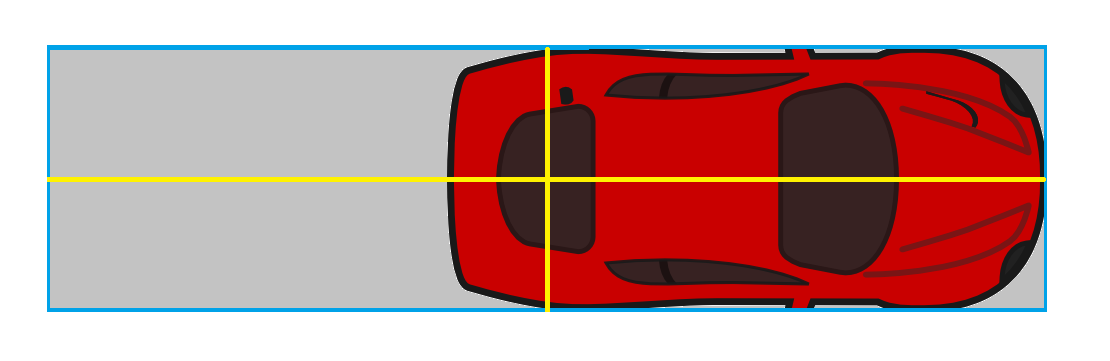
\includegraphics[width=0.9\textwidth]{car_image_explained_3}
    \caption{The car image with transparency in non car areas \label{fig:visualisation_module:car_image_explained_3} }
\end{figure}

\subsubsection{Loading Vehicle Images}

At the initialization of the VisualisationModule class, the vehicle images are loaded. The loading process consists in accessing the image file and loading into memory, and afterwards resize it so that the image has the correct dimensions for the SML World visualisation window.

The image is first loaded using \texttt{pygame.image.load}, and afterwards rescaled using \texttt{pygame.transform.smoothscale}. In order to find the new image size, we simply convert the car width into the corresponding pixel distance in the visualisation window. The ratio between the original image height and the car width in pixels gives us the resizing ratio. This resizing ratio is then applied the original image, both in the height and width dimensions. We now have a car image with a scale appropriate to the visualisation window.

The method implementing this procedure is \texttt{load\_vehicle\_image} in the VisualisationModule class. This method is used by several load functions, like \texttt{load\_red\_car\_image}, \texttt{load\_truck\_image}, \texttt{load\_big\_box\_image} and \texttt{load\_goal\_image}.

\subsubsection{Drawing Vehicles}

To draw a vehicle we need its state $(x,y,\theta)$. The first step consists in rotating the vehicle image, so that it matches the current vehicle $\theta$. This is achieved using \texttt{pygame.transform.rotate}, which returns a new image with the vehicle rotated. Due to the restrictions imposed on the vehicle image creation (see \ref{visualisation_module:creating_vehicle_images}), the center of the rotated image will still correspond to the car rear axle.

We then get the pixel position $(p_x,p_y)$ corresponding to the car position. The rotated image is then placed at $(p_x - \frac{width}{2}, p_y - \frac{height}{2})$. This guarantees that the vehicle's rear axle will be positioned at $(p_x,p_y)$, as desired.

The \texttt{draw\_vehicle\_image} method implements this functionality. This method is called by other methods such as \texttt{draw\_red\_car}, \texttt{draw\_truck}, \texttt{draw\_big\_box} and \texttt{draw\_goal}.

\subsubsection{Drawing Ids}

For many purposes it might be necessary to show the vehicle ids next to the corresponding vehicles. The ids are drawn next to the vehicles if the VisualisationModule's attribute \texttt{show\_ids} is set to \texttt{True}, otherwise they are not.

The id drawing functionality is implemented by the \texttt{draw\_id} method.

\subsubsection{Drawing the next frame}

pygame's image display is based on the \texttt{pygame.Surface.blit} process. \textit{Blitting} consists in drawing one image on top of another.

In order to show the environment and the vehicles in it we first need to blit the environment (background) image onto the Visualisation Window. Afterwards, we need to blit all of the vehicles onto the Visualisation Window, this results in the Visualisation Window displaying the environment and the vehicles in it.

In order to draw a new frame, with vehicles in different places, we need to remove the previously placed vehicles and then draw the new ones. Unfortunately it is impossible to remove the vehicles once they have been blitted onto the visualisation window, so the solution consists in blitting the whole background image once again onto the Visualisation Window, effectively cleaning all of the vehicles. The new vehicles are then blitted once again on top of this clean background image.

When blitting the whole environment image, we are effectively blitting many regions with no vehicles on it. This means that blitting in this regions is useless, since it will simply replace the old pixels with new pixels with the same values. In order to try to remove some of this unecessary, and expensive, blitting, a "smart blitting" is implemented. 

The smart blitting tries to blit only in regions that are indeed necessary to blit. To do so, every time a vehicle is drawn, we store in memory the region where the vehicle was drawn. In the next frame, instead of blitting the whole background, we simply blit the background in the stored regions, corresponding to the places where vehicles are drawn. This results in less areas being blitted, and it was observed that it resulted in less computational expense.

This blitting technique might become more expensive than the whole background blitting if there are a big number of vehicles in the image. To date this was not noticed. But it is the belief of the author that there is the possibility of this happening. The concern is that it might be less expensive to blit one region of $x^2$ pixels, than blitting a big number of regions with a combined area smaller than $x^2$ pixels.

\subsection{Threading restrictions}
\label{visualisation_module:threading_restrictions}

pygame requires the main thread of the program in order to do event handling and render the graphics, this would mean that the VisualisationModule would have to run in the main thread of the SML World.Since we would like to have pygame running on it's own independent thread, the solution found was to use the \texttt{multiprocessing} module to create a new python process which would run the Visualisation Module and give pygame the main thread of this process. This solution was based on the suggestion given in \cite{pygame_threading}.

Since the Visualisation Module is now running on a separate process, it cannot have access to the SML World memory, like the other modules have. However, the Visualisation Module requires only the vehicle states to draw them, and this information can be sent via messages, as explained in the following section.

\subsection{Interfacing with the SML World}

The Visualisation Module needs information about the SML World, namely the vehicles to draw. To get this information, and remembering, that we do not have direct access to the SML World, and the vehicles in it, we set up a UDP connection between the SML World and the Visualisation Module. Currently this communication channel is only one way and it consists in vehicle states being sent from the SML World to the Visualisation Module.

Remembering \ref{fig:visualisation_module_diagram} we know that this communications is made making use of the classes Visualisation Module Sender and Visualisation Module Receiver. 

The Visualisation Module Sender class, is a class that will loop on its own thread, and its task consists in creating and sending the UDP messages containing the vehicle information to the Visualisation Module. This class is instantiated by the SML World, and has a reference to it, being able to interact with the Vehicles Dictionary containing the information about the vehicles.

The class constructor takes as arguments \texttt{visualisation\_address} and \texttt{desired\_rate}. The first corresponds to the IP of the computer running the Visualisation Module, it can be \texttt{\'localhost\'} if the module is running on the same computer, or a standard IP address, if one wishes to have the Visualisation Module running on another computer. \texttt{desired\_rate} defines the frequency at which messages will be sent to the Visualisation Module. 

Similarly to the Sender class, the Visualisation Module Receiver class will also loop on its own thread, however this class is instantiated by the Visualisation Module. The Receiver class is responsible for receiving and parsing the UDP messages sent by the Sender class. The parsed information corresponds to the relevant information about the vehicles present in the SML World.

A typical UDP message exchanged between contains the information about all the vehicles in the SML World. The information about each vehicle consists of the id of the vehicle, the state $(x,y,\theta)$, and the class name. The class name allows us to know which kind of vehicle we are drawing, car, truck or even obstacles. For more details about the format of the exchanged message and the parsing of it, one should look at the implementation details in the class code.

Each UDP message also has a packet number, which is used to compensate for the unreliability of the UDP protocol. Every time a message is sent from the Sender Module, a packet number is added to the message. The packet number starts at 1, and it increases by 1 at each message. This allows the Receiver Module, to know if it is receiving the packets in the correct order, and in case it is not, it will issue a warning via terminal to the user, and ignore said packet.


\section{The Motion Capture Module}
\label{sec:the_motion_capture_model}



\section{The Real Trucks Module}
\label{sec:the_real_trucks_module}


\graphicspath{ {SectionInstallationGuide/} }

\section{Installation Guide}
\label{sec:installation_guide}

This section guides the reader through the installation of the necessary software in order to start using the SML World. It will first focus on the installation of Python and afterwards on the additional Python libraries required for the SML World to run.

The instructions are targeted for a Windows system. The SML World is also able to run in Unix systems, as long as Python and the required libraries are installed. A guide for installing in Unix systems is not provided, as we assume that a Unix user should be able to easily understand the Windows Installation procedure, and will have not trouble in adapting it to his own system.

\subsection{Python Installation and Setup}

The SML World was developed using Python 2.7. In order to run Python programs you need to install the software available at \url{https://www.python.org/downloads/}. Select Python version $2.7.x$ as shown in figure \ref{fig:python_install_download}

\begin{figure}[h!]
  \centering
    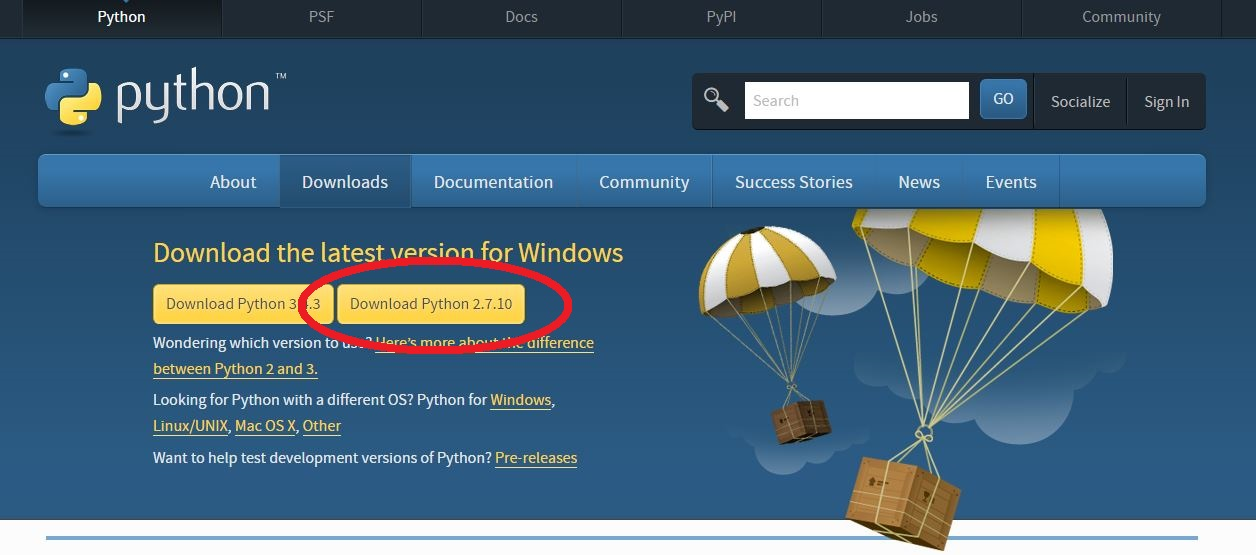
\includegraphics[width=0.6\textwidth]{python_install_1}
    \caption{Downloading Python $2.7.x$ \label{fig:python_install_download} }
\end{figure}


Right click the downloaded file and select Install. Follow the installation instructions, and when you arrive at the window shown in figure \ref{fig:python_install_option_add_path}, select “Will be installed on local drive” for the \textit{Add python.exe to Path} option.

\begin{figure}[h!]
  \centering
    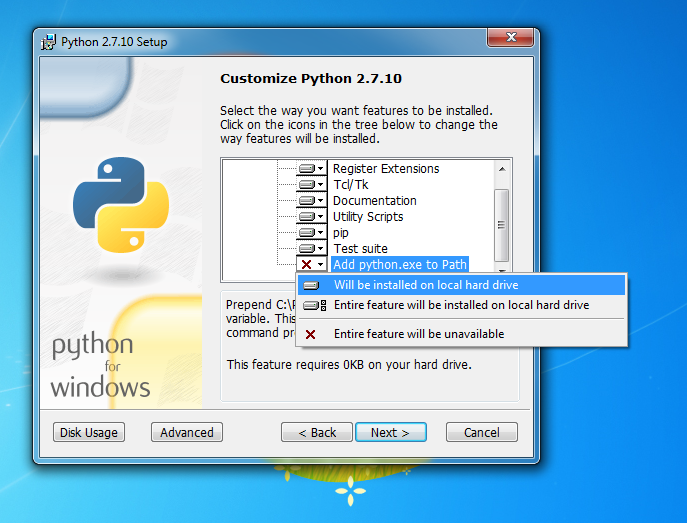
\includegraphics[width=0.6\textwidth]{python_install_3}
    \caption{Adding Python to the System Path \label{fig:python_install_option_add_path} }
\end{figure}

Press next, and the installation will continue, and eventually finish. To test if Python was successfully installed, simply open a terminal (to do so, open the Start Menu, and write \texttt{cmd} in the search bar, and click \texttt{cmd.exe}, figure \ref{fig:python_install_open_terminal}), and enter the command \texttt{python}. The result should be the one shown in figure \ref{fig:python_install_python_command}. If it is, you can jump to section \ref{subsec:installing_python_libraries}  and start installing the Python libraries.

If you cannot replicate the result seen in the figure, and instead get the message \texttt{'python' is not recognized as an internal or external command, operable program or batch file}, then go to section \ref{subsec:adding_python_to_environment_path}.

\begin{figure}[h!]
  \centering
    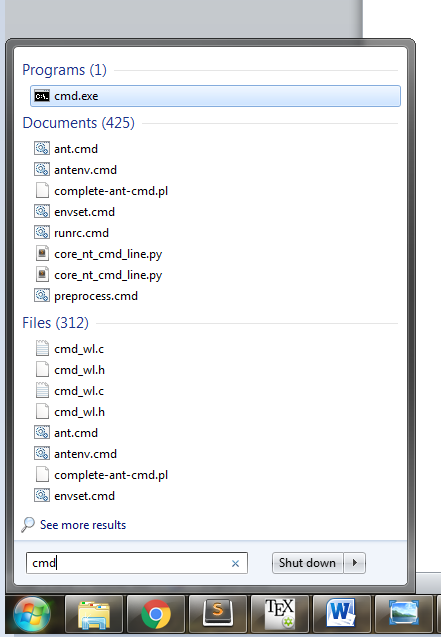
\includegraphics[width=0.6\textwidth]{python_install_opening_terminal}
    \caption{Opening a terminal \label{fig:python_install_open_terminal} }
\end{figure}


\begin{figure}[h!]
  \centering
    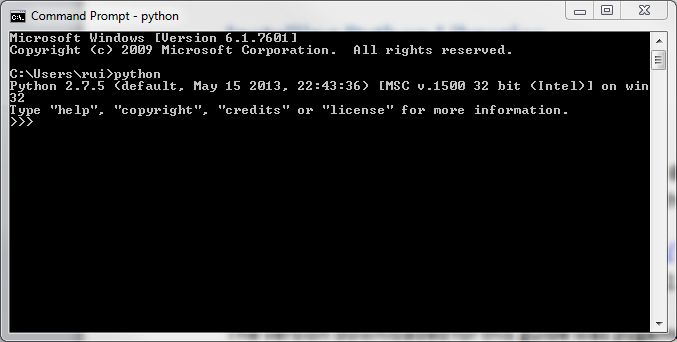
\includegraphics[width=0.9\textwidth]{python_install_terminal_python_command}
    \caption{Running the \texttt{python} command \label{fig:python_install_python_command} }
\end{figure}

\subsection{Manually Adding Python To Environment Path}
\label{subsec:adding_python_to_environment_path}

If you installed Python, but cannot run it, then the reason might be that Python was not added to the windows Path variable. This Path variable, contains information about the location of programs, so that they can be called/run from the command line.

The first thing to do is to find where your Python installation folder is located. If you followed the default installation steps, then your Python folder should be at \texttt{C:\\Python27}, as seen in figure \ref{fig:python_install_python_folder}. If it is not there, try to locate it in other possible folders (suggestions: \texttt{ProgramFiles}, \texttt{ProgramFiles (x86)}).

\begin{figure}[h!]
  \centering
    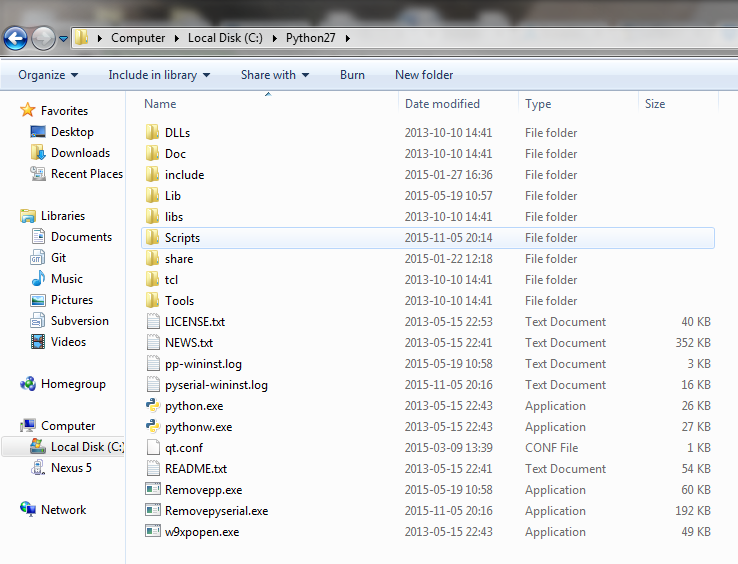
\includegraphics[width=0.9\textwidth]{python_install_python_folder}
    \caption{The python installation folder \label{fig:python_install_python_folder} }
\end{figure}

Now that you located the folder where \texttt{python.exe} is, you need to add it to the Windows Path Variable. To do so, open the Windows Menu, and type \texttt{var} in the search bar, then select \texttt{Edit the system environment variables}, as seen in figure \ref{fig:python_install_opening_environment_variables}.


\begin{figure}[h!]
  \centering
    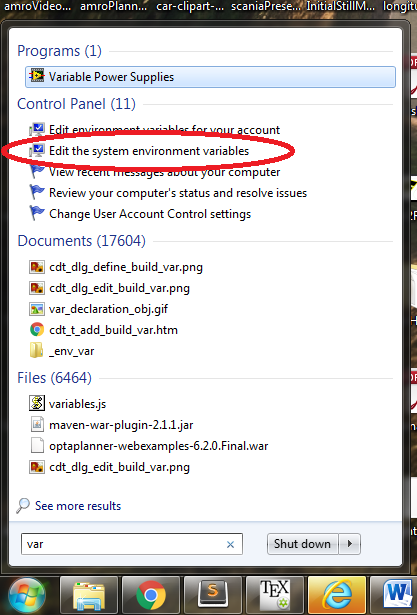
\includegraphics[width=0.6\textwidth]{python_install_4}
    \caption{Opening the System Environment Variables \label{fig:python_install_opening_environment_variables} }
\end{figure}

The \texttt{System Properties} window will open, press \texttt{Environment Variables...}, in the new window, find the \texttt{path} variable, and click \texttt{Edit...} (in case the \texttt{path} variable does not exist you will need to create it by pressing \texttt{New...}). A new window appears, now you simply have to add the folder path of the Python folder, simply add \texttt{C:\\Python27} (or another directory where you installed Python), with a preceding semicolon to separate it from other paths that might already be there. Figure \ref{fig:python_install_adding_to_the_path_variable} shows this process. In this case the Python location is between two other locations, so it has a semicolon before and another after.

\begin{figure}[h!]
  \centering
    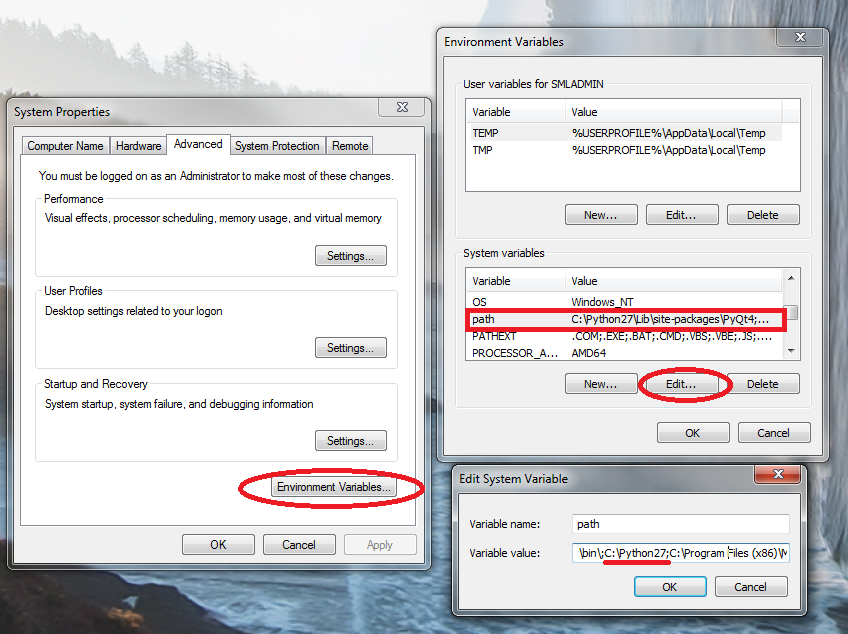
\includegraphics[width=0.9\textwidth]{python_install_6_highlighted}
    \caption{Editing the Path Variable \label{fig:python_install_adding_to_the_path_variable} }
\end{figure}

Close the terminal and reopen it (necessary so that it uses the new System Variable Path). Type Python, you should now be able to see figure \ref{fig:python_install_python_command}.

\subsection{Installing Additional Python Libraries}
\label{subsec:installing_python_libraries}

Python libraries are modules that provide python with specific high level programming commands, that allow the user to develop code with less effort and bigger productivity.

\subsubsection{Installing pygame}

Pygame is a library that allows the programmer to develop nice graphical visualisations with ease. This library is used by the Visualisation and Road Modules in order to display and generate the SML World environment.

Pygame can be found in \url{http://www.pygame.org/}. Simply go to the Downloads page, and select the correct pygame version for your Python version (2.7).
The version downloaded for this guide was \texttt{pygame-1.9.1.win32-py2.7.msi} (3.1MB). Simply run the file, and install using all the default installation settings.

\subsubsection{Installing NumPy}

The NumPy library provides the developer with mathematical tools that can be useful in a large number of situations.

To install it you will need to access \url{http://www.lfd.uci.edu/~gohlke/pythonlibs/}, 

and go to the NumPy section
 \url{http://www.lfd.uci.edu/~gohlke/pythonlibs/\#numpy}.
 You should download the .whl file that suits your python and computer version, in this tutorial \texttt{numpy-1.9.2+mkl-cp27-none-win32.whl} is used. The \texttt{27} in the filename indicates that this is numpy for the Python 2.7 version.

Open the terminal in the folder where the file we just downloaded is located. You can do it by simply pressing \texttt{SHIFT+RIGHT CLICK} and then pressing Open command window here, see figure \ref{fig:numpy_install_open_terminal}.

\begin{figure}[h!]
  \centering
    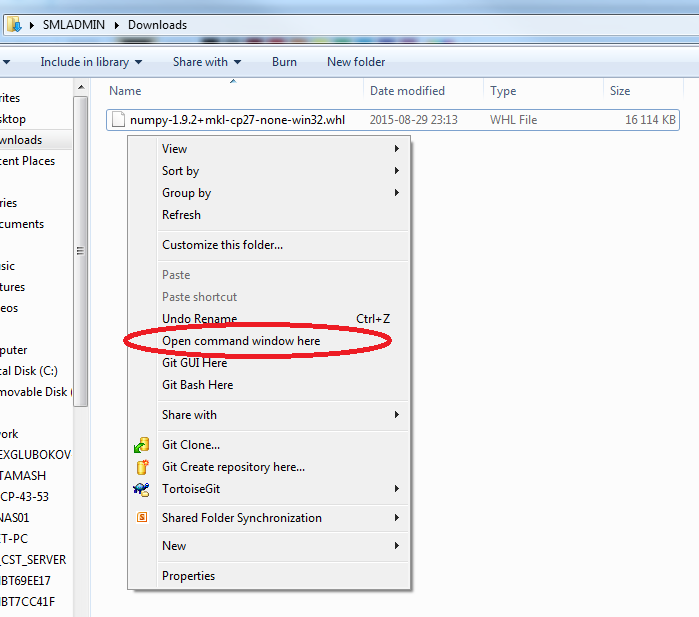
\includegraphics[width=0.9\textwidth]{numpy_install_open_terminal_highlighted}
    \caption{Opening the terminal in a folder location \label{fig:numpy_install_open_terminal} }
\end{figure}

In the terminal that opens run the command \texttt{pip install \"numpy-1.9.2+mkl-cp27-none-win32.whl\"}. This will call Python's \texttt{pip} program that allows for an easy installation of Python libraries. 

\begin{figure}[h!]
  \centering
    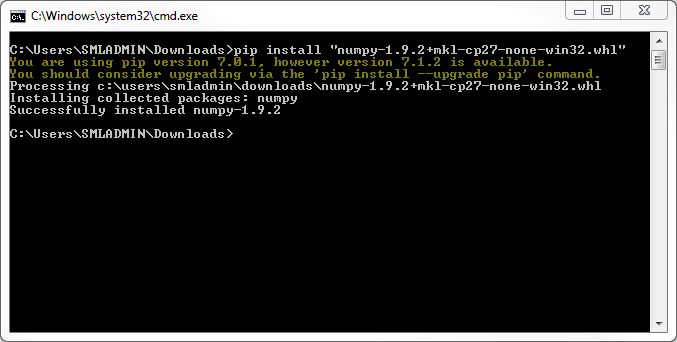
\includegraphics[width=0.9\textwidth]{numpy_install_success}
    \caption{Successful installation of NumPy using \texttt{pip install} \label{fig:numpy_install_success} }
\end{figure}

If you get the error \texttt{'pip' is not recognized as an internal or external command, operable program or batch file}, then you need to add \texttt{pip} to the Environment Variable Path (see section \ref{subsubsec:adding_pip_to_path}).

If the installation was sucessful, like shown in image \ref{fig:numpy_install_success}, then go to section \ref{subsubsec:installing_shapely}.

\subsubsection{Adding Pip to Environment Path}
\label{subsubsec:adding_pip_to_path}

The \texttt{pip} program is included in the current versions of the Python installer. To check that you have it in your system simply go to the Python installtion folder, and check the \texttt{Scripts} folder in it, it should contain an executable \texttt{pip.exe}. To be able to run \texttt{pip install} from the command line you need to add this folder to the System Variable Path. The process is the same as the one explained in section \ref{subsec:adding_python_to_environment_path}, however instead of adding the Python folder location we add the Python\\Scripts folder location, as seen in figure \ref{fig:pip_install_environment_variable}.

\begin{figure}[h!]
  \centering
    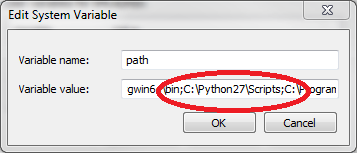
\includegraphics[width=0.7\textwidth]{pip_install_environment_variable_highlighted}
    \caption{Adding \texttt{pip} to variable Path \label{fig:pip_install_environment_variable} }
\end{figure}

To test that you successfully added \texttt{pip} to the System Variable Path simply close and reopen the terminal, and type the command \texttt{pip install}. You should see have the same result as figure \ref{fig:pip_install_test}.

\begin{figure}[h!]
  \centering
    \includegraphics[width=0.9\textwidth]{pip_install_test}
    \caption{Successful installation of \texttt{pip} \label{fig:pip_install_test} } 
\end{figure}

\subsubsection{Choosing the correct .whl File}
\label{subsubsec:choosin_whl_file}

\subsubsection{Installing Shapely}
\label{subsubsec:installing_shapely}

Shapely is currently only being used by the Blockly Module. You only need to install it in case you pretend to run the SML School code. Shapely is a module that allows for simple handling and operation of geometric objects.

Similarly to NumPy, it can be downloaded and installed using \texttt{pip install}. First download Shapely from \url{http://www.lfd.uci.edu/~gohlke/pythonlibs/#shapely}. In this guide the downloaded file was \texttt{Shapely-1.5.12-cp27-none-win32.whl}. The installation process is identical to NumPy's installation. 



\section{Contributors and Development}
\label{sec:Contributors}

The SML World is a project started in January 2015 by João Pedro Alvito and Rui Oliveira, under the supervision of Pedro Lima and Jonas Mårtensson.

Until May 2015 the main focus of development of the SML World was directed towards the iQMatic demonstration at Scania.

After this demonstration the development started to shift towards platooning and cooperative driving solutions. From June to August the SML World team welcomed the contributions of four students from the ACCESS Summer Projects. Elin Karlsson and Johan Clemedson developed Platooning oriented controllers for the scaled trucks present at the SML, while Felix Abrahamsson and Magnus Arvidsson implemented perception and supervisory modules aiming to solve some of the challenges of the GCDC 2016 competition.



\section{Previous Versions and Abandoned Modules}

\begin{thebibliography}{9}

\bibitem{OSM}
OpenStreetMap Wiki \url{http://wiki.openstreetmap.org/wiki/Main_Page}

\bibitem{JOSM}
JOSM \url{https://josm.openstreetmap.de/}

\bibitem{pygame}
pygame \url{www.pygame.org/}

\bibitem{GIMP}
GIMP \url{http://www.gimp.org/}

\bibitem{no-ip}
NO-IP \url{http://www.noip.com/}


\end{thebibliography}


\end{document}